
%% bare_conf.tex
%% V1.4b
%% 2015/08/26
%% 作者:迈克尔·谢尔
%% 参见:
%% http://www.michaelshell.org/
%%用于当前联系信息。
%%
%%这是演示互联网。cls使用情况的骨架文件
%%（需要IEEE.cls版本1.8 b或更高版本）具有IEEE
%% 会议论文。
%%
%%支持站点:
%% http://www.michaelshell.org/tex/ieeetran/
%% http://www.ctan.org/pkg/ieeetran
%%和
%% http://www.ieee.org/

%%*************************************************************************
%%法律声明:
%%此代码按原样提供，不提供任何明示或暗示的保证。
%%隐含；甚至不包含适销性的隐含保证或
%%适合特定用途！
%%用户承担所有风险。
%%在任何情况下，IEEE或本代码的任何贡献者均不对
%%任何损害或损失，包括但不限于附带的，
%%因使用或误用而导致的后果性或任何其他损害
%%。
%%
%%所有评论均为其各自作者的意见，并非
%%必须得到IEEE的认可。
%%
%%本作品在LaTeX（LaTeX）项目公共许可证（LPPL）下发行
%%(http://www.latex-project.org/）1.3版，并且可以自由使用，
%%已分发和修改。包含1.3版LP PL的副本
%%
%% 2003/12/01或更晚。
%%保留所有捐款通知和信用额。
%% ** 修改后的文件应明确标明，包括**
%% ** 重命名它们并更改作者支持联系信息. **
%%*************************************************************************


% *** 作者应验证（并在需要时纠正）他们的LaTeX系统***
% *** 在信任他们的LaTeX平台之前使用测试流诊断***
% *** 涉及生产工作。IEEE的字体选择和纸张尺寸可***
% *** 触发在使用其他类文件时不会出现的错误.       ***                          ***
%测试流支持页面位于:
% http://www.michaelshell.org/tex/testflow/



\documentclass[conference]{{IEEEtran}}
%某些计算机协会会议也要求使用compsoc模式选项，
%但其他使用标准会议格式。
%
%如果互联网.cls没有安装到LaTeX系统文件中，
%手动指定通向它的路径，如:
% \documentclass[conference]{../sty/IEEEtran}


%一些非常有用的LaTeX包包括：
%（取消评论您要加载的内容）


% *** 杂项实用包 ***
%
%\使用包{ifpdf}
%海科的if pdf.sty非常有用，如果你需要有条件的话。
%编译基于输出是pdf还是dvi。
%使用率:
% \ifpdf
%   % PDF代码
%\否则
%   % 数字图像编码（DVI）代码
% \fi
%if pdf.sty的最新版本可从以下位置获取：
% http://www.ctan.org/pkg/ifpdf
%另外，请注意互联网.cls V 1.7及更高版本提供了内置的
%\如果条件，其工作方式相同。
%当从乳胶切换到PDFlatex，反之亦然时，编译器可能会
%必须运行两次才能清除警告/错误消息。






% *** 签名包 ***
%
%\使用软件包
%cite.sty由唐纳德阿瑟诺撰写
%V1.6及更高版本预定义了citrate.sty包的格式
%\cite{}输出遵循IEEE输出。加载引用包将
%导致引文编号被自动和正确地排序
%"压缩/分区"。例如，[1], [9], [2], [7], [5], [6]不使用
%cit.sty将变成[1], [2], [5]--[7], [9]使用网站。
%\cite将在需要时自动添加引号。使用cite.sty的
%无调整选项（参照.sty V3.8及更高版本）如果您想关闭此选项
%例如，如果引文需要附在括号内。
%cita.sty已安装在大多数LaTeX系统上。请确保并使用
%版本5.0（2009-03-20）及更高版本（如果使用hyperref.sty）。
%可在以下网址获取最新版本:
% http://www.ctan.org/pkg/cite
%文档包含在cite.sty文件中。






% *** 图形相关包裹 ***
%

% 
  %声明图形文件所在的路径
  % \图形path{{../pdf/}{../jpeg/}}
  %及其扩展，因此您不必指定这些扩展。
  % 每个 \includegraphics 实例
  % \DeclareGraphicsExtensions{.pdf,.jpeg,.png}

  %或其他类选项（dvipsone，dvipdf，如果不使用dvips）。graphicx
%将默认使用系统图形.cfg中指定的驱动程序
  % driver is specified.
  % \usepackage[dvips]{graphicx}
  % declare the path(s) where your graphic files are
  % \graphicspath{{../eps/}}
  % and their extensions so you won't have to specify these with
  % every instance of \includegraphics
  % \DeclareGraphicsExtensions{.eps}

% graphicx was written by David Carlisle and Sebastian Rahtz. It is
% required if you want graphics, photos, etc. graphicx.sty is already
% installed on most LaTeX systems. The latest version and documentation
% can be obtained at: 
% http://www.ctan.org/pkg/graphicx
% Another good source of documentation is "Using Imported Graphics in
% LaTeX2e" by Keith Reckdahl which can be found at:
% http://www.ctan.org/pkg/epslatex
%
% latex, and pdflatex in dvi mode, support graphics in encapsulated
% postscript (.eps) format. pdflatex in pdf mode supports graphics
% in .pdf, .jpeg, .png and .mps (metapost) formats. Users should ensure
% that all non-photo figures use a vector format (.eps, .pdf, .mps) and
% not a bitmapped formats (.jpeg, .png). The IEEE frowns on bitmapped formats
% which can result in "jaggedy"/blurry rendering of lines and letters as
% well as large increases in file sizes.
%
% You can find documentation about the pdfTeX application at:
% http://www.tug.org/applications/pdftex





\usepackage{geometry} % 调整页边距（可选）
\geometry{a4paper, scale=0.8}
\usepackage{booktabs}
\usepackage{tikz} 
\usepackage{float}
\IEEEoverridecommandlockouts


\usetikzlibrary{shapes,arrows,positioning,fit,calc}
\usepackage{amsmath}  % 数学公式核心包
\usepackage{amssymb}  % 数学符号包
\usepackage{graphicx} % 插入图片包
\usepackage{algorithm} % 算法伪代码包
\usepackage{booktabs} % 三线表
\usepackage{float}    % 强制图片位置
\usepackage{algpseudocode}
\usepackage{multirow} 
\usepackage{longtable}
\usepackage{enumitem}
\usepackage{algorithm}
\usepackage{algpseudocode}
\usepackage{amsmath}
\usepackage{float}  % 用于 [H] 强制固定位置
\usepackage{booktabs}
\usepackage{amsmath}

% *** MATH PACKAGES ***
%
%\usepackage{amsmath}
% A popular package from the American Mathematical Society that provides
% many useful and powerful commands for dealing with mathematics.
%
% Note that the amsmath package sets \interdisplaylinepenalty to 10000
% thus preventing page breaks from occurring within multiline equations. Use:
%\interdisplaylinepenalty=2500
% after loading amsmath to restore such page breaks as IEEEtran.cls normally
% does. amsmath.sty is already installed on most LaTeX systems. The latest
% version and documentation can be obtained at:
% http://www.ctan.org/pkg/amsmath





% *** SPECIALIZED LIST PACKAGES ***
%
%\usepackage{algorithmic}
% algorithmic.sty was written by Peter Williams and Rogerio Brito.
% This package provides an algorithmic environment fo describing algorithms.
% You can use the algorithmic environment in-text or within a figure
% environment to provide for a floating algorithm. Do NOT use the algorithm
% floating environment provided by algorithm.sty (by the same authors) or
% algorithm2e.sty (by Christophe Fiorio) as the IEEE does not use dedicated
% algorithm float types and packages that provide these will not provide
% correct IEEE style captions. The latest version and documentation of
% algorithmic.sty can be obtained at:
% http://www.ctan.org/pkg/algorithms
% Also of interest may be the (relatively newer and more customizable)
% algorithmicx.sty package by Szasz Janos:
% http://www.ctan.org/pkg/algorithmicx




% *** ALIGNMENT PACKAGES ***
%
%\usepackage{array}
% Frank Mittelbach's and David Carlisle's array.sty patches and improves
% the standard LaTeX2e array and tabular environments to provide better
% appearance and additional user controls. As the default LaTeX2e table
% generation code is lacking to the point of almost being broken with
% respect to the quality of the end results, all users are strongly
% advised to use an enhanced (at the very least that provided by array.sty)
% set of table tools. array.sty is already installed on most systems. The
% latest version and documentation can be obtained at:
% http://www.ctan.org/pkg/array


% IEEEtran contains the IEEEeqnarray family of commands that can be used to
% generate multiline equations as well as matrices, tables, etc., of high
% quality.




% *** SUBFIGURE PACKAGES ***
%\ifCLASSOPTIONcompsoc
%  \usepackage[caption=false,font=normalsize,labelfont=sf,textfont=sf]{subfig}
%\else
%  \usepackage[caption=false,font=footnotesize]{subfig}
%\fi
% subfig.sty, written by Steven Douglas Cochran, is the modern replacement
% for subfigure.sty, the latter of which is no longer maintained and is
% incompatible with some LaTeX packages including fixltx2e. However,
% subfig.sty requires and automatically loads Axel Sommerfeldt's caption.sty
% which will override IEEEtran.cls' handling of captions and this will result
% in non-IEEE style figure/table captions. To prevent this problem, be sure
% and invoke subfig.sty's "caption=false" package option (available since
% subfig.sty version 1.3, 2005/06/28) as this is will preserve IEEEtran.cls
% handling of captions.
% Note that the Computer Society format requires a larger sans serif font
% than the serif footnote size font used in traditional IEEE formatting
% and thus the need to invoke different subfig.sty package options depending
% on whether compsoc mode has been enabled.
%
% The latest version and documentation of subfig.sty can be obtained at:
% http://www.ctan.org/pkg/subfig




% *** FLOAT PACKAGES ***
%
%\usepackage{fixltx2e}
% fixltx2e, the successor to the earlier fix2col.sty, was written by
% Frank Mittelbach and David Carlisle. This package corrects a few problems
% in the LaTeX2e kernel, the most notable of which is that in current
% LaTeX2e releases, the ordering of single and double column floats is not
% guaranteed to be preserved. Thus, an unpatched LaTeX2e can allow a
% single column figure to be placed prior to an earlier double column
% figure.
% Be aware that LaTeX2e kernels dated 2015 and later have fixltx2e.sty's
% corrections already built into the system in which case a warning will
% be issued if an attempt is made to load fixltx2e.sty as it is no longer
% needed.
% The latest version and documentation can be found at:
% http://www.ctan.org/pkg/fixltx2e


%\usepackage{stfloats}
% stfloats.sty was written by Sigitas Tolusis. This package gives LaTeX2e
% the ability to do double column floats at the bottom of the page as well
% as the top. (e.g., "\begin{figure*}[!b]" is not normally possible in
% LaTeX2e). It also provides a command:
%\fnbelowfloat
% to enable the placement of footnotes below bottom floats (the standard
% LaTeX2e kernel puts them above bottom floats). This is an invasive package
% which rewrites many portions of the LaTeX2e float routines. It may not work
% with other packages that modify the LaTeX2e float routines. The latest
% version and documentation can be obtained at:
% http://www.ctan.org/pkg/stfloats
% Do not use the stfloats baselinefloat ability as the IEEE does not allow
% \baselineskip to stretch. Authors submitting work to the IEEE should note
% that the IEEE rarely uses double column equations and that authors should try
% to avoid such use. Do not be tempted to use the cuted.sty or midfloat.sty
% packages (also by Sigitas Tolusis) as the IEEE does not format its papers in
% such ways.
% Do not attempt to use stfloats with fixltx2e as they are incompatible.
% Instead, use Morten Hogholm'a dblfloatfix which combines the features
% of both fixltx2e and stfloats:
%
% \usepackage{dblfloatfix}
% The latest version can be found at:
% http://www.ctan.org/pkg/dblfloatfix




% *** PDF, URL AND HYPERLINK PACKAGES ***
%
%\usepackage{url}
% url.sty was written by Donald Arseneau. It provides better support for
% handling and breaking URLs. url.sty is already installed on most LaTeX
% systems. The latest version and documentation can be obtained at:
% http://www.ctan.org/pkg/url
% Basically, \url{my_url_here}.




% *** Do not adjust lengths that control margins, column widths, etc. ***
% *** Do not use packages that alter fonts (such as pslatex).         ***
% There should be no need to do such things with IEEEtran.cls V1.6 and later.
% (Unless specifically asked to do so by the journal or conference you plan
% to submit to, of course. )


% correct bad hyphenation here
\hyphenation{op-tical net-works semi-conduc-tor}
\raggedbottom



%
% paper title
% Titles are generally capitalized except for words such as a, an, and, as,
% at, but, by, for, in, nor, of, on, or, the, to and up, which are usually
% not capitalized unless they are the first or last word of the title.
% Linebreaks \\ can be used within to get better formatting as desired.
% Do not put math or special symbols in the title.
\title{A Combined BiTCN-Attention-KAN and Sand Cat Swarm Optimization Framework for Energy-SLA Balanced VM Migration in Cloud Data Centers
}


% author names and affiliations
% use a multiple column layout for up to three different
% affiliations
\author{Jie Li, Yu Wu
\thanks{
        % 下面这段内容会自动出现在首页左下角红框位置
        J. Li and Y. Wu are with the School of Artificial Intelligence, South China Normal University, Foshan, Guangdong 528225, China (e-mail: lijie@m.scnu.edu.cn; 2024024538@m.scnu.edu.cn).
    }
}

% conference papers do not typically use \thanks and this command
% is locked out in conference mode. If really needed, such as for
% the acknowledgment of grants, issue a \IEEEoverridecommandlockouts
% after \documentclass

% for over three affiliations, or if they all won't fit within the width
% of the page, use this alternative format:
% 
%\author{\IEEEauthorblockN{Michael Shell\IEEEauthorrefmark{1},
%Homer Simpson\IEEEauthorrefmark{2},
%James Kirk\IEEEauthorrefmark{3}, 
%Montgomery Scott\IEEEauthorrefmark{3} and
%Eldon Tyrell\IEEEauthorrefmark{4}}
%\IEEEauthorblockA{\IEEEauthorrefmark{1}School of Electrical and Computer Engineering\\
%Georgia Institute of Technology,
%Atlanta, Georgia 30332--0250\\ Email: see http://www.michaelshell.org/contact.html}
%\IEEEauthorblockA{\IEEEauthorrefmark{2}Twentieth Century Fox, Springfield, USA\\
%Email: homer@thesimpsons.com}
%\IEEEauthorblockA{\IEEEauthorrefmark{3}Starfleet Academy, San Francisco, California 96678-2391\\
%Telephone: (800) 555--1212, Fax: (888) 555--1212}
%\IEEEauthorblockA{\IEEEauthorrefmark{4}Tyrell Inc., 123 Replicant Street, Los Angeles, California 90210--4321}}




% use for special paper notices
%\IEEEspecialpapernotice{(Invited Paper)}


\begin{document}

% make the title area
\maketitle

% As a general rule, do not put math, special symbols or citations
% in the abstract
\begin{abstract}
Optimizing virtual machine (VM) migration is paramount for enhancing energy efficiency and resource utilization in dynamic cloud data centers. However, aggressive VM migration often exacerbates resource contention, leading to critical Service Level Agreement (SLA) violations. Existing models frequently overlook this delicate balance, prioritizing energy reduction while neglecting SLA integrity, and often rely on suboptimal centralized allocation schemes. To address these challenges, this paper proposes , a novel BiTCN-ATTENTION-KAN (BAK) based prediction and Sand Cat Swarm Optimization (SCSO) driven VM migration framework termed BAK-SCSO-VMM, which introduces BiTCN-ATTENTION-KAN, a  neural network model, to accurately predict VM energy consumption by effectively capturing multi-variable correlations, temporal features, and non-linear relationships through flexible curve fitting inherent in Kolmogorov-Arnold Network (KAN). Building upon these predictions, a dynamic VM allocation algorithm powered by SCSO is designed to intelligently explore optimal VM configurations that balance energy saving with SLA adherence. The experimental results demonstrate that BAK-SCSO-VMM achieves significant energy efficiency gains from 16.1\%  to 21.9\% over the LSTM and TCN benchmarks, respectively, while restricting the SLA violation rate to a mere 0.0165\%. Furthermore, our approach exhibits superior adaptability and robust generalization performance across diverse VM scales.

\end{abstract}

% no keywords
% 关键词部分 (在这里！)
  \begin{IEEEkeywords}
    VM migration (VMM), Cloud data centers, Energy consumption prediction, BiTCN, Sand Cat Swarm Optimization (SCSO), Service Level Agreement (SLA)
  \end{IEEEkeywords}

% For peer review papers, you can put extra information on the cover
% page as needed:
% \ifCLASSOPTIONpeerreview
% \begin{center} \bfseries EDICS Category: 3-BBND \end{center}
% \fi
%
% For peerreview papers, this IEEEtran command inserts a page break and
% creates the second title. It will be ignored for other modes.
\IEEEpeerreviewmaketitle
\section{introduction}
% no \IEEEPARstart
With the upgrading of the global digital industry and the large-scale development of artificial intelligence, both the number and scale of data centers have witnessed explosive expansion\cite{lou2025hybrid}.  According to a report by the International Energy Agency (IEA), global energy consumption accounted for about 2\% of total electricity consumption in 2022, approximately 460 TWh\cite{adegboye2024dgs}. It is speculated that this figure may increase to around 1,000 TWh by 2026 and will continue to rise in the foreseeable future. Energy consumption and related carbon emissions have become the main obstacles hindering the sustainable development of data centers\cite{torquato2025evaluation}. Consequently, implementing robust energy management strategies that reconcile power reduction with high-performance service delivery has become an imperative research priority.

To mitigate excessive energy consumption, Virtual Machine (VM) migration and integration technologies have been extensively explored by both academia and industry. By leveraging virtualization, a single PM can concurrently support multiple VM instances, significantly enhancing hardware utilization compared to traditional one-to-one mapping architectures\cite{mondal2024multi}. Within this domain, dynamic VM migration stands out as a critical strategy, underpinned by live migration technology\cite{chongdarakul2024heuristic}. This approach enables the intelligent reallocation of VMs to PMs based on resource demands. Consequently, underutilized physical machines can be transitioned into sleep or shutdown states, thereby minimizing idle power consumption and optimizing the overall energy footprint of the data center.

Despite these advancements, contemporary VM migration technologies remain suboptimal\cite{mondal2024multi}. The Service Level Agreement (SLA) defines critical performance benchmarks—such as bandwidth guarantees and latency thresholds—that service providers must uphold. An escalation in SLA violation rates not only degrades user experience but also exposes providers to substantial financial penalties and reputational damage. Beyond these risks, current integration strategies suffer from three primary limitations: 

1) Most existing migration frameworks are reactive. They initiate VM migrations only after performance bottlenecks are detected, by which time the SLA has frequently been breached. 

2) Conventional models often focus exclusively on CPU utilization while neglecting memory dynamics\cite{lou2025hybrid}\cite{mondal2024multi}. This narrow focus can lead to deceptive results where low CPU usage masks high memory swap rates, ultimately causing system performance to collapse. 

3) While previous deep learning models, such as Temporal Convolutional networks (TCN), exhibit parallel computing advantages in capturing local features, they typically rely on fixed convolution kernels for the final output. This architectural constraint prevents them from accurately predicting sudden, non-linear workload spikes, resulting in significant underestimation during dynamic fluctuations..

Without achieving proactive adaptation and multi-dimensional resource awareness, data centers will continue to struggle with the conflicting objectives of minimizing energy consumption and maintaining stringent SLA compliance.

To address the aforementioned limitations, this paper proposes a synergized framework called BAK-SCSO-VMM, which integrates advanced deep learning for proactive prediction with a robust swarm intelligence algorithm for VM migration. Specifically, we develop the BiTCN-ATTENTION-KAN (BAK) model to accurately predict  energy consumption\cite{chua2024building}. While the Bidirectional Temporal Convolutional Network (BiTCN) excels at capturing long-term temporal dependencies from historical data\cite{paul2024optimizing}, it shares a common structural flaw with LSTM: the reliance on linear output layers. To overcome this, we incorporate the Kolmogorov-Arnold Network (KAN) with an attention mechanism. By utilizing learnable, non-linear activation functions on edges rather than fixed nodes, KAN provides an arbitrarily flexible curve-fitting capability. This allows the model to capture both subtle stabilities and sharp, non-linear fluctuations in VM energy consumption, facilitating proactive resource management such as timely transitioning idle PMs into sleep mode\cite{bresson2024kagnns}\cite{mondal2024multi}.

For the VM migration phase, we employ the Sand Cat Swarm Optimization (SCSO) algorithm to determine the optimal VM migration scheme\cite{ajmera2024dynamic}. To enhance its search efficiency, a Lens Imaging Learning (LIL) mechanism is integrated into the SCSO algorithm. The LIL mechanism effectively prevents the population from being trapped in local optima by diversifying the search space, thereby ensuring the discovery of a global optimal solution for energy-SLA balancing\cite{yang2025cam}. The integration of BAK-driven prediction and LIL-SCSO-based allocation enables a more efficient, adaptive, and proactive approach to cloud resource optimization. The main contributions of this paper are summarized as follows:

\begin{itemize}
    \item  We design the BAK-SCSO-VMM framework, a novel BiTCN-ATTENTION-KAN (BAK) model based prediction and Sand Cat Swarm Optimization (SCSO) algorithm driven VM migration. By integrating Bidirectional Temporal Convolutional Networks (BiTCN) with the Kolmogorov-Arnold Network (KAN), the framework effectively captures long-term temporal dependencies and multi-variable correlations to predict energy consumption.

    \item  BAK-SCSO-VMM incorporates an intelligent VM migration algorithm powered by Sand Cat Swarm Optimization (SCSO). This algorithm utilizes the predictive insights from the BAK model to explore a global search space of VM configurations.

    \item  Through extensive simulations using the Cloudsim toolkit, we demonstrate the superiority of the proposed BAK-SCSO-VMM framework. The results reveal that BAK-SCSO-VMM achieves an energy efficiency improvement of 21.9\% and 16.1\% compared to LSTM and TCN benchmarks, respectively, while maintaining a remarkably low SLA violation rate of 0.0165\%, proving its robust generalization across diverse data center scales.
\end{itemize}

The rest of this paper is organized as follows. Section II reviews the related work. Section III builds the system model . Section IV details the design of BAK-SCSO-VMM. Section V reports the performance evaluation results. Finally, Section VII concludes the paper and outlines directions for future research.

\section{related work}
\subsection{Research on VM Energy Consumption Prediction}

Accurate prediction of PM energy consumption over subsequent time intervals forms the foundation of proactive resource management. Detecting workload peaks enables timely provisioning of reliable resources to prevent SLA violations\cite{ranganna2024fitness}\cite{chua2024building}, while identifying energy consumption troughs allows PMs to transition to low-power sleep modes\cite{altahat2025virtual}. Therefore, energy consumption prediction is at the core of the data center resource management.

Traditional cloud energy consumption predicting primarily relied on conventional statistical models, most prominently autoregressive integrated moving average (ARIMA). These methods assume a linear relationship between historical and future data\cite{boroumand2025heuristic}, modeling CPU utilization as a linear trajectory\cite{elhabyb2024machine}. While ARIMA offers exceptional computational efficiency and minimal hardware overhead, it is fundamentally constrained by its linear assumptions. Real-world cloud traffic is typically random and nonlinear, characterized by sudden traffic surges driven by external events. In such scenarios, linear models fail to capture underlying chaotic patterns, leading to severe prediction inaccuracies.

To address nonlinear problems, classical machine learning methods such as Support Vector Regression (SVR)\cite{ciampi2024energy} and Random Forest (RF)\cite{abualigah2024improved} are introduced. SVR utilizes kernel functions to map low-dimensional inputs to high-dimensional feature spaces, enabling recognition of complex patterns. Conversely, RF employs ensembles of decision trees to simultaneously handle heterogeneous features like CPU and memory\cite{yang2025cam}\cite{adegboye2024dgs}. Despite enhanced flexibility, these approaches remain heavily reliant on manual feature engineering. Moreover, in the face of an extremely large amount of constantly changing data, the time dependence of machine learning methods in obtaining past time data and present data are very poor\cite{du2024metaheuristic}. The advent of Recurrent Neural Networks (RNNs)\cite{boroumand2025heuristic} marked a shift toward automated feature extraction. However, RNNs suffer from the vanishing gradient problem, which limits their long-term memory capabilities. Long Short-Term Memory (LSTM)\cite{noorizadegan2025practitioner}\cite{zhang2024optimizing} networks mitigate this issue by introducing gate mechanisms that selectively retain or discard information. While LSTMs have dominated energy consumption predicting for years, their inherently serial architecture precludes parallel computation, resulting in excessively long training times.

To enhance computational throughput, Temporal Convolutional Networks (TCNs)\cite{wu2024hotspot} are proposed. By employing dilated convolutions, TCNs achieve extended receptive fields and support parallel processing. However, TCNs assign equal importance to all historical data points, lacking the focusing capability required to distinguish critical events from routine fluctuations.

The above studies have a certain role in improving throughput and achieving automatic feature extraction, but they seldom consider the impact of the VM energy consumption in combination with focusing capability. In our study, our BAK-SCSO-VMM assigns varying weights to energy consumption to identify key events and prioritizes their processing to minimize total energy consumption.

\subsection{Research on Virtual Machine Migration}

Effective VM migration is the critical phase following energy consumption predicting. Its purpose is to map a large number of VMs to physical machines (PMs) in a manner that minimizes energy consumption while mitigating SLA violations\cite{lella2024towards}.

In the nascent stages of cloud computing, scheduling strategies primarily relied on simple heuristic algorithms such as First Fit (FF)\cite{du2024metaheuristic} . The FF algorithm sequentially scans PMs and assigns VMs to the first node with sufficient remaining capacity. While computationally efficient, FF is inherently “short-sighted” and greedy. This strategy frequently leads to severe resource fragmentation, where the idle capacity accumulated across multiple PMs is insufficient to accommodate larger tasks. This necessitates activating additional nodes and results in persistently high energy consumption\cite{song2024predicting}.

To overcome the limitations of local search, swarm intelligence algorithms inspired by nature are widely adopted. For instance, Particle swarm optimization (PSO)\cite{rhif2023veg} mimics the foraging patterns of bird flocks, where particles adjust their trajectories based on the fastest “leader.” While PSO exhibits rapid convergence, it is prone to “premature convergence” in high-dimensional VMM problems, where the leader may stagnate at suboptimal solutions, causing the entire swarm to deviate.

Recent advancements have introduced more powerful meta-heuristic algorithms, such as the Grey Wolf Optimizer (GWO))\cite{bresson2024kagnns} and Sandcat Swarm Optimization (SCSO)\cite{qasim2024chaotic}. SCSO simulates the hunting process of felines in arid environments, alternating between “carpet-style” global search and refined “local search” based on sensitive auditory cues. However, when applied to large-scale computing clusters, SCSO frequently encounters population diversity stagnation. To address this issue, we introduced Lens Imaging Learning (LIL)\cite{ranganna2024fitness}. To address the issue of SCSO easily getting stuck in local optima when processing data, Lens Imaging Learning strategy is introduced. By utilizing optical imaging principles, an opposite solution is generated, forcing the population to look in the opposite direction. This enables the algorithm to escape from the current local optimum and explore unexplored areas, thereby enhancing its ability to find the global optimum. The SCSO algorithm employs lens imaging principles to generate reverse candidate solutions, preventing the population from prematurely converging on local sandpits (local optima). This forces the population to explore uncharted regions of the search space to obtain superior global solutions.

\section{system model}

\subsection{System Framework Overview}

We furnished the BAK-SCSO-VMM as a software infrastructure that allows PM to realize energy optimization for data centers.  Fig.1  elaborates the system architecture diagram of managing resources of data centers using the proposed framework. The proposed framework consists of two core modules: energy consumption prediction using the BiTCN-Attention-KAN, and VM migration decision using the improved Sand Cat Swarm Optimization algorithm (SCSO-LIL). These components work synergistically to dynamically optimize resource allocation of physical hosts, minimizing total energy consumption and significantly reducing Service Level Agreement violations (SLAV). First, the Workload Monitor is responsible for the real-time collection of CPU utilization and relevant memory metrics from both physical machines (PMs) and VMs.  In the Prediction Module, the BiTCN-Attention-KAN model is used to predict the energy consumption status of the next time interval, enabling the proactive identification of PM overloads. Third, for the Decision and Optimization Module, an improved SCSO-LIL algorithm is employed to generate a globally optimal VM migration strategy based on the predictive insights.  Finally, the Execution Module is tasked with implementing the generated migration plans and updating the global resource status accordingly.Our framework is responsible for the migration and migration of VMs to PMs of the data center based on the prediction and optimization models. We model the cloud data center as a set containing $N$ PMs $H=\{h_{1}, h_{2}, ..., h_{N}\}$.  Considering that many different indicators are involved in practice,  each PM differs in the number of CPU cores,  memory capacity, and bandwidth. The VM set is represented as $V=\{v_{1}, v_{2}, ..., v_{M}\}$.  The objective for $V$ is to find an optimal placement matrix $X$ = \begin{equation}
X = 
\begin{bmatrix}
    X_1 \\
    X_2 \\
    \vdots \\
    X_N
\end{bmatrix}
=
\begin{bmatrix}
    x_{1,1} & x_{1,2} & \cdots & x_{1,D} \\
    x_{2,1} & x_{2,2} & \cdots & x_{2,D} \\
    \vdots  & \vdots  & \ddots & \vdots \\
    x_{N,1} & x_{N,2} & \cdots & x_{N,D}
\end{bmatrix}
\label{eq:population_matrix}
\end{equation} at a certain moment $t$,  where $x_{ij}=1$ indicates that VM $v_i$ is placed on PM $h_j$.  This search process is subject to a hard constraint on the quantity of physical machines,  that is,  the resource demand of all VMs on a single PM is exceed the upper limit of that PM.
\begin{figure*}[!t] % 加星号表示跨双栏，[!t] 强制置顶
    \centering
    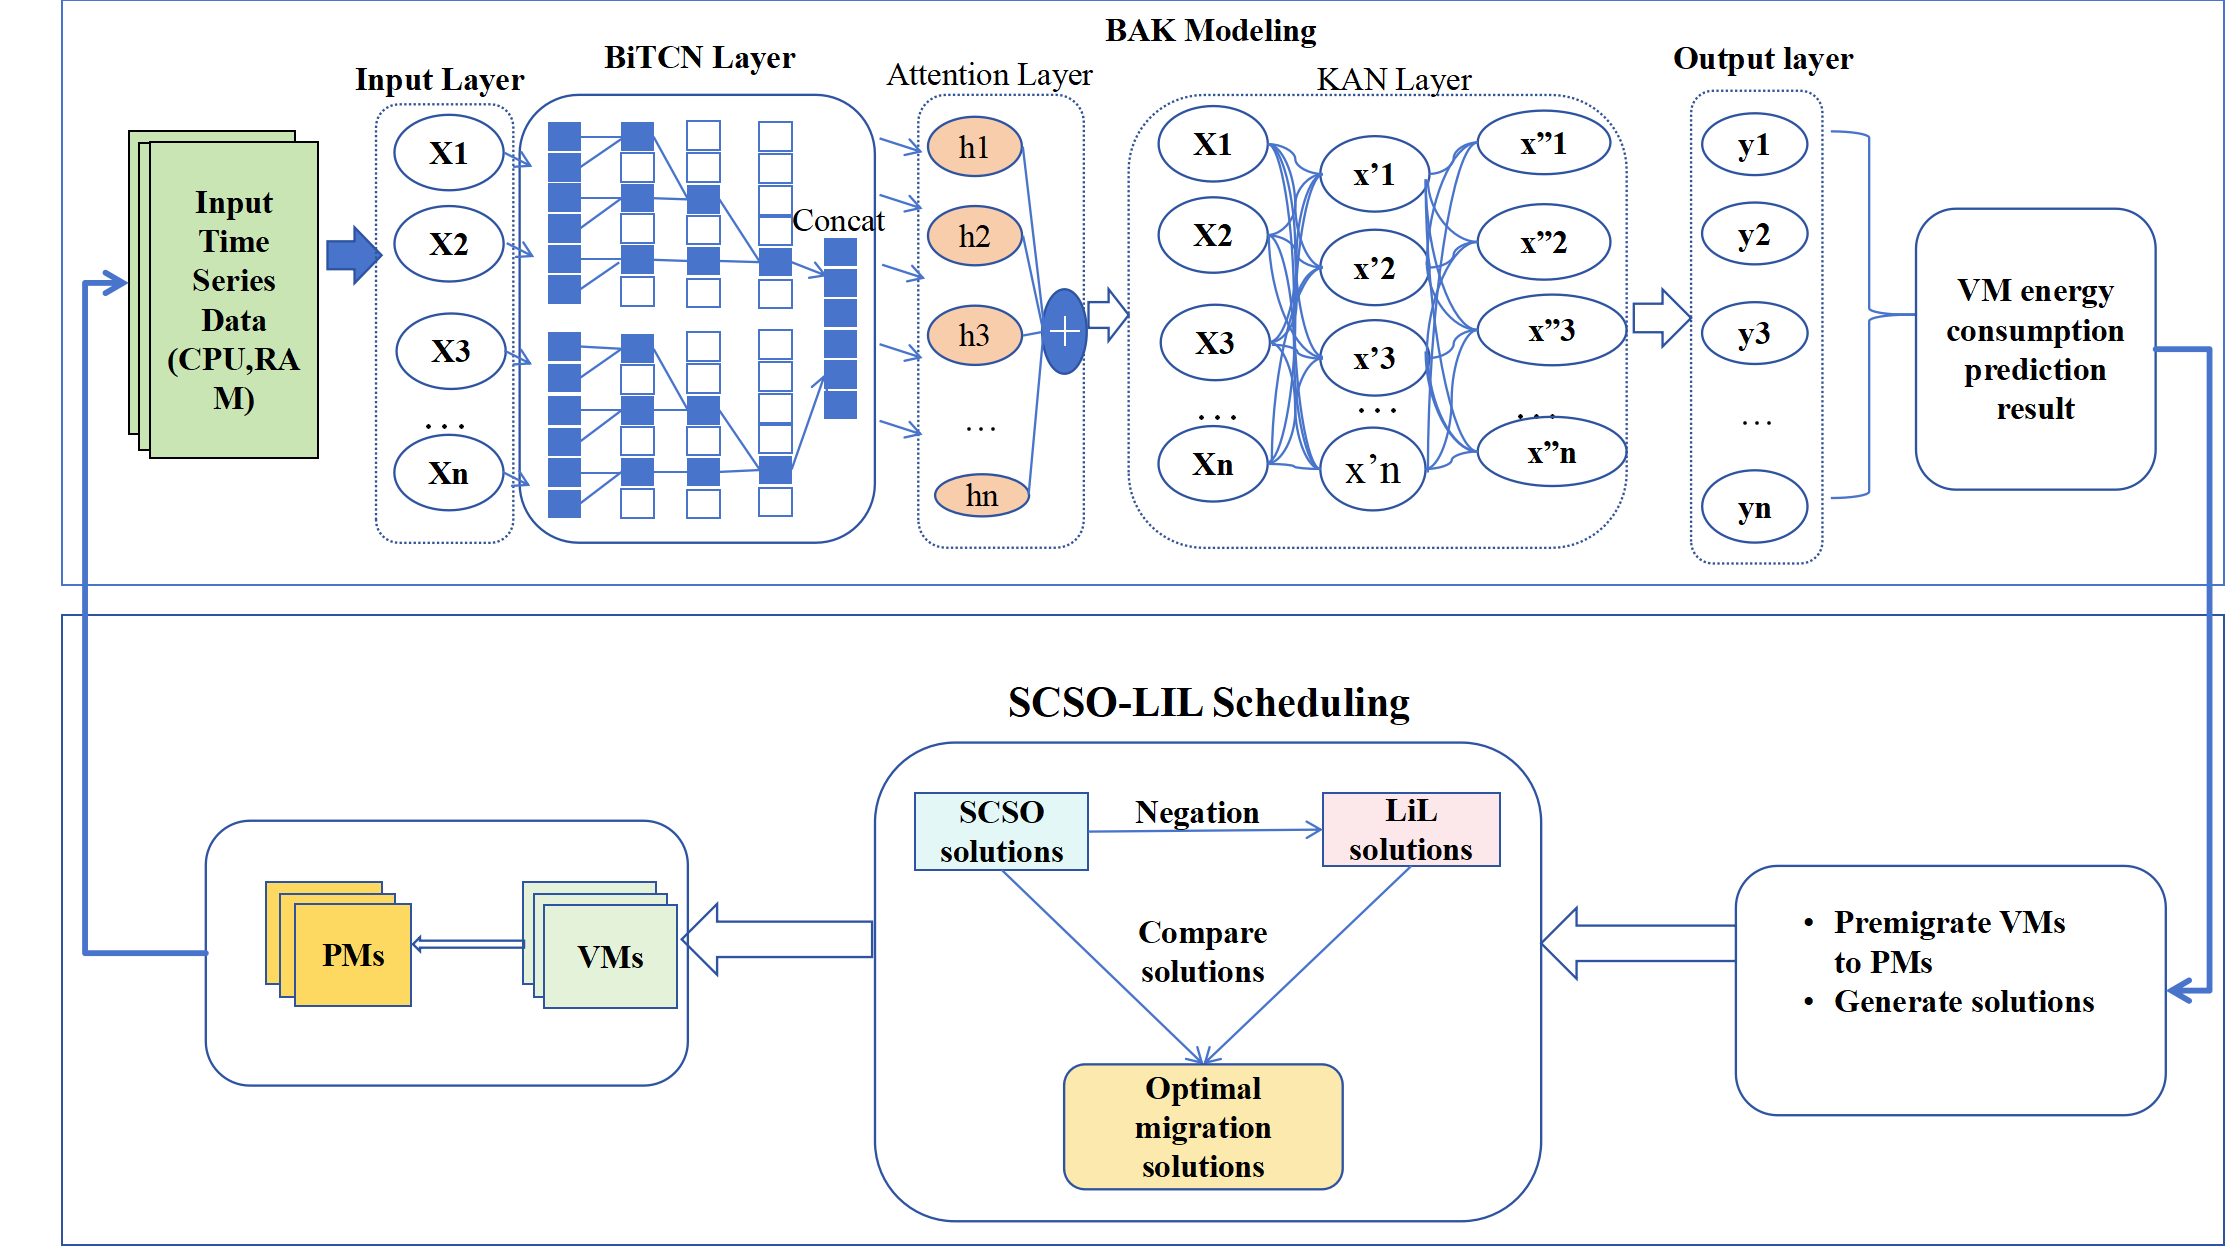
\includegraphics[width=0.95\textwidth]{IEEEtran/Overall System.png} 
    % 注意：跨栏图建议将 columnwidth 改为 textwidth，以获得更好的视觉宽度
    \caption{Overall System diagram}
    \label{fig:model_structure}
\end{figure*}

\subsection{PM Energy and SLA Violation Model}

In a cloud computing environment, the energy consumption of PM is not simply summed up. Relevant studies indicates\cite{torquato2025evaluation} that the CPU is the part with the largest proportion of energy consumption in the PM, and the relationship between its power consumption and resource utilization is not a simple linear one. Current models often misjudge the sudden increase in energy consumption under high loads. For example, when dealing with high-load inputs, LSTM exhibits insensitivity to energy consumption fluctuations at load levels exceeding 90\%, leading to misjudgments. Furthermore, ARIMA is inadequate for high-load forecasting; for example, the accuracy of energy consumption predictions for loads between 90\% and 95\% declines much more sharply than it does under low-load conditions. Therefore, the energy consumption prediction model adopted in this study depicts the instantaneous power $P_i(t)$ of the PM $h_{i}$ at a certain moment as the sum of the reference power consumption in the non-operating state and the power consumption in the high-load operating state. Specifically, even if the current PM is not overloaded, it still consumes about 70\% of its maximum power. This is to ensure the normal standby of the PM's hardware such as the motherboard fan, hard drive, and network interface. When the CPU utilization rate increases due to the current load, power consumption  increases exponentially\cite{cui2024energy}. This also indicates a key solution: if you want to minimize energy consumption, the most direct method is to use integration technology to concentrate VMs on as few PMs as possible, so that more idle PMs can enter sleep or shut down states.The calculation formula of  $P_i(t)$ is as follows:\begin{equation}
    P_i(t) = k \cdot P_{max} + (1-k) \cdot P_{max} \cdot u_i(t)^\gamma,
\label{eq:power_model}
\end{equation}
where $P_i(t)$ represents the real-time power consumption of the i-th PM at time $t$, $P_{max}$ is the maximum power when the PM is operating at full capacity, $k$ is the idle power coefficient, which is the proportion of the PM's energy consumption in the idle state (utilization rate of 0) to its maximum energy consumption, $u_i(t)$ represents the current CPU utilization rate, and $\gamma$ is a nonlinear calibration parameter used to more accurately calculate the nonlinear relationship between load and power consumption in actual scenarios (if $\gamma=1$, it degenerates to a linear model).

However, relying solely on the energy consumption model (Fig.1) for resource scheduling is insufficient. Specifically, when the PMs becomes overloaded and cannot provide sufficient CPU clock cycles or memory required by the VMs, the lack of underlying resources directly result in the blocking of computational tasks and increased response delays, ultimately leading to Service Level Agreement (SLA) violations. To precisely calculate this potential performance loss while minimizing energy consumption. The SLA violation rate (SLAV) has been established as a key constraint metric, measuring system stability in terms of time. When the CPU utilization rate of a certain physical machines (PMs) reaches 100\%, it indicates that the physical machine is in an overloaded state. SLATAH is defined as the ratio of the time all PMs are in an overloaded state to their running time. This metric reflects the negative effects brought about by integration, that is, the higher the degree of integration, the greater the probability of overload, which leads to a higher SLATAH.\begin{equation}
    SLATAH = \frac{1}{N} \sum_{i=1}^{N} \frac{T_{o,i}}{T_{a,i}},
    \label{eq:slatah}
   \end{equation}
where $N$ represents the total number of active PMs, $T_{o,i}$ is the total time that the $i$-th PM is at 100\% CPU utilization, and $T_{a,i}$ is the total active running time of that PM. The overall formula calculates the average proportion of time that all PMs are unable to provide normal services due to overload.

To eliminate overload situations or integrate resources, the system needs to constantly migrate VMs\cite{liu2025impact}. However, the migration process itself is not completely energy-free. Migration consumes additional CPU cycles to write dirty pages in memory back to the hard disk. PDM (Performance Degradation due
to Migration) quantifies the overall performance degradation caused by VM migration.
\begin{equation}
    PDM = \frac{1}{M} \sum_{j=1}^{M} \frac{C_{d,j}}{C_{r,j}},
    \label{eq:pdm}
    \end{equation}
where PDM (Performance Degradation due to Migration) measures the average percentage of performance degradation caused by virtual machine migration, $M$ represents the total number of VMs undergoing migration, $C_{d,j}$ is the performance estimation value of the performance loss caused by the $j$-th virtual machine during the migration process, and $C_{r,j}$ is the total capacity requested or allocated by that virtual machine. The overall calculation of the formula is the average negative impact of all migration operations on virtual machine performance.

    Combining the above two points, the Service violation Rate (SLAV) is defined as the product of SLATAH and PDM:\begin{equation}
    SLAV = SLATAH \times PDM
    \label{eq:slav}
\end{equation}
This definition indicates that SLAV approaches zero only when both system stability (SLATAH) and migration dropout (PDM) are optimized under non-overloaded conditions. Therefore, the objective of this study is to seek the overall minimum value between total energy consumption (Etotal) and violation rate (SLAV) while meeting more resource-intensive requirements.


\subsection{BiTCN-Attention-KAN (BAK) model}

The current resource management models all use threshold-type passive trigger mechanisms (for example, migration is only triggered when the CPU exceeds 80\%). This kind of post-event handling strategy has a very high lag. It is often only taken after the system has suffered extremely severe congestion or caused very high energy consumption. In order to achieve a shift from passive response to active management, accurately predicting future energy consumption trends is of great significance. However, the energy consumption vector of cloud data centers has a very high degree of instability and volatility. Existing models such as LSTM or TCN, although performing well in handling stationary situations, often fail in prediction due to the linear idleness of their prediction functions when facing sudden energy consumption changes in cloud computing.
For this situation, we present the model: BiTCN-Attention-KAN.
\begin{figure}[!t]
    \centering
    
    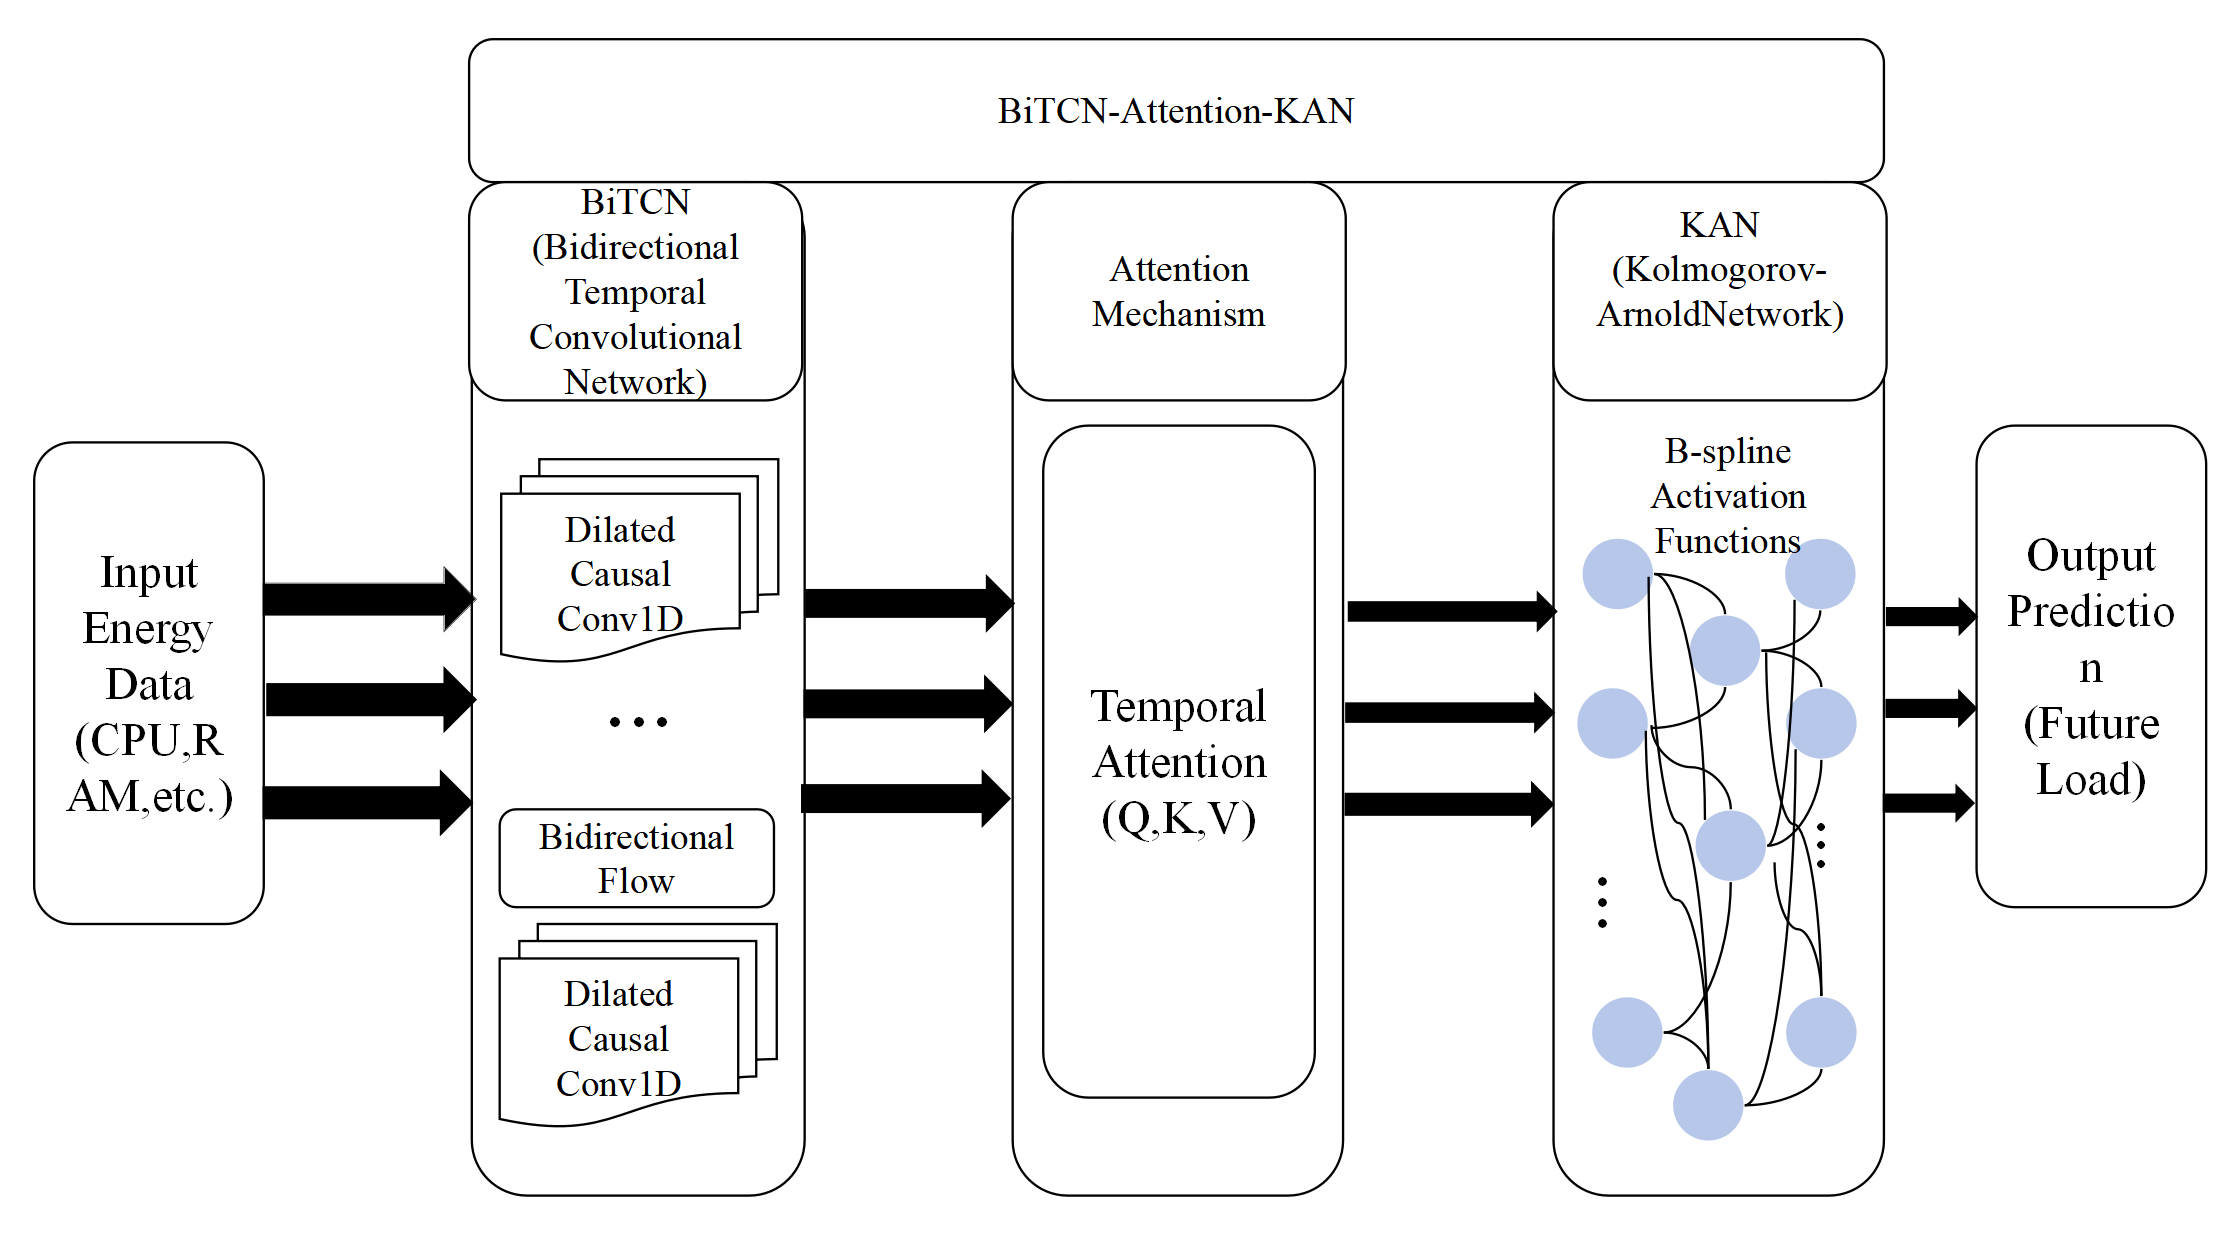
\includegraphics[width=0.95\columnwidth]{model_structure.png}
    \caption{BiTCN-Attention-KAN model}
    \label{fig:model_structure}
\end{figure}
Figure 2 illustrates the architecture of the BiTCN-Attention-KAN  prediction model. Considering the nonlinear characteristics and reliance on past time data during cloud computing, a three-layer core structure has been designed. First, the data is input into the BiTCN layer, which uses a convolutional model to extract the features of the time series to predict future energy consumption. Then, the feature vectors enter the Attention layer, where different weights are dynamically assigned to each vector through the attention mechanism to identify and focus on the past time points and nearby time points that have the greatest impact on future loads, such as sudden load points\cite{lella2024towards}. Finally, the KAN layer is used, and the edge functions within it are utilized for efficient nonlinear mapping to output the final predicted resource demand situation. This end-to-end design significantly enhances the ability of the model in this study to predict energy consumption in complex and variable situations in reality.

\subsection{Sand Cat Swarm Optimization (SCSO) Model}

SCSO is a population algorithm that learns the way sand cats use low-frequency noise to find food. This algorithm achieves an adaptive adjustment from carpet-style search to local refined search through the sand cat's auditory sensitivity regulation mechanism. The algorithm introduces a sensitivity parameter $r_G$ which is used to calculate the auditory sensitivity
rG of the sand cat:\begin{equation}
    r_G = s_M - \left( \frac{s_M \times t}{T_{\max}} \right),
    \label{eq:scso_sensitivity}
\end{equation}
where $s_M$ represents the maximum sensitivity constant, $t$ denotes the current iteration count, and $T_{max}$ signifies the preset maximum total iteration count. As the iteration process progresses (i.e., $t$ gradually increases), this formula causes $r_G$ to linearly decrease from $s_M$ to 0, thereby guiding the algorithm's focus to smoothly transition from wide-area global search in the early stages to local precise exploitation in the later stages.

As the number of iterations continuously increases, $r_G$ gradually decreases, which represents simulating the auditory focus situation of the sand cat when approaching prey.  When $|R| > 1$ (where $R = 2r_G \times \text{rand} - r_G$), the sand cat relies on the current best position and other individuals' positions, take an overall average value, and then move to that average value position before conducting a random search.
    
When $|R| \le 1$, the sand cat approaches the food through its super-sensitive hearing. At this time, it conducts a refined search:
\begin{equation}
    X_{new} = 
    \begin{cases} 
    % 第一种情况：拆分为两行
    \begin{aligned}
        &\frac{X_{best} + X_{centroid}}{2} + \\
        &r_G \cdot (X_{curr} - X_{rand}) 
    \end{aligned} 
    & |R| > 1 \quad \\
  % 增加一点垂直间距
    \\[5pt]   
    % 第二种情况：拆分为两行
    \begin{aligned}
        &X_{best} - r_G \cdot \text{rand} \cdot \\
        &\cos(\theta) \cdot (X_{best} - X_{curr})
    \end{aligned} 
    & |R| \le 1 \quad,
    \end{cases}
    \label{eq:scso_update}
\end{equation}

\section{Algorithm Design of the BAK-SCSO-VMM}

\subsection{Energy Prediction by the BiTCN-Attention-KAN model}

Tasks issued by clients are enclosed in one or more VMs, and some hot tasks replicate themselves in multiple VMs to cope with failures. We postulated that a single VM executes a single task, and the VM terminates after the task is executed. It is noteworthy that the task is encapsulated in the VM. Thus, our approach is independent of the type of task. We considered processing tasks by PM in data centers as the allocation of PMs by VMs (e.g. CPU and Memory). To achieve energy reduction, we introduce the Bidirectional Temporal Convolutional Network (BiTCN) to capture the temporal correlation of energy consumption. BiTCN employs a causal dilation convolution mechanism, ensuring that prediction relies only on past data, while utilizing its expansibility to sample data from relatively distant positions in the input sequence. The output of its residual block is as follows:
\begin{equation}
    H_l(t) = \text{ReLU}\left( \sum_{k=0}^{K-1} w_k \cdot H_{l-1}(t - k \cdot d_l) + b \right),
    \label{eq:dilated_conv}
\end{equation}
where $H_l(t)$ and $H_{l-1}$ denote the output vector of the $l$-th layer at time step $t$ and the input sequence of the $(l-1)$-th layer, respectively,  $w_k$ and $b$ represent the weight parameters and bias term of the convolution kernel,  $d_l$ is the dilation factor of the layer determining the sampling interval of the kernel,  $K$ is the kernel size, while BiTCN can extract rich temporal features, its output layer is usually a linear layer, which leads to a decline in the model's processing ability for nonlinear data\cite{zhang2025predicting}. Therefore, Attention-KAN is integrated into BiTCN to enhance performance.

\begin{algorithm}[!t] 
\caption{Training Process of the BiTCN Energy Consumption Prediction Model}
\label{alg:bitcn_training}
\begin{algorithmic}[1]
% --- 输入输出 ---
\State \textbf{Input:} Historical energy consumption sequence $\mathcal{D}$, Sliding window size $w$, Learning rate $\eta$, Maximum Epochs $K$.
\State \textbf{Output:} Trained neural network parameters $\Theta^*$.

% --- 步骤 1: 初始化 ---
\State \textbf{Step 1: Initialization}
\State Initialize network weights $W$ and biases $b$ (Xavier initialization);
\State Preprocess data: Normalize $\mathcal{D}$ to $[0, 1]$ and create sliding windows;

% --- 步骤 2: 训练循环 ---
\State \textbf{Step 2: Training Loop}
\While{$k < K$ and not converged}
    \For{each mini-batch $(X_b, Y_b)$ in Training Set}
        \State // \textbf{Forward Propagation}
        \State $F_{fwd} \leftarrow \text{DilatedConv1D}(X_b)$; \Comment{Forward features}
        \State $F_{bwd} \leftarrow \text{DilatedConv1D}(\text{Reverse}(X_b))$; \Comment{Backward features}
        \State $H_{comb} \leftarrow \text{Concat}(F_{fwd}, F_{bwd})$; \Comment{Feature Fusion}
        \State $\hat{Y}_b \leftarrow \text{FullyConnected}(H_{comb})$;
        
        \State // \textbf{Backpropagation}
        \State Compute Loss $\mathcal{L} = \text{MSE}(\hat{Y}_b, Y_b)$;
        \State Calculate gradients $\nabla_\Theta \mathcal{L}$;
        \State Update parameters: $\Theta \leftarrow \Theta - \eta \cdot \text{Adam}(\nabla_\Theta \mathcal{L})$;
    \EndFor
    \State Validate model performance on Validation Set;
    \State $k \leftarrow k + 1$;
\EndWhile

\State \textbf{Return} Optimized parameters $\Theta^*$.
\end{algorithmic}
\end{algorithm}

In the feature sequence extracted by BiTCN, not all historical data information has significant reference value and meaning\cite{song2024predicting}. For instance, when predicting the maximum value of a single energy consumption, the weights of adjacent data from the previous few seconds and similar peak data from the past should be much higher than those during the stable period\cite{bi2023network}.

The calculation is defined as follows:\begin{equation}
        \text{Attention}(Q, K, V) = \text{softmax}\left(\frac{Q K^T}{\sqrt{d_k}}\right) V,
        \label{eq:attention}
    \end{equation}
where $Q$, $K$, and $V$ represent the current query vector, the indexing features used for retrieval, and the actual content information, respectively,  The context vectors, weighted by the Attention mechanism, are directly fed into the KAN layer to capture intricate inter-data relationships. Derived from the Kolmogorov-Arnold representation theorem, KAN places learnable activation functions on the edges (weights) of the network connections. Specifically, each path in the KAN is represented as a variable function rather than a simple scalar weight. During training, these functions adapt their shapes and control points based on the input distribution. In stable phases, the functions approximate linear shapes\cite{rhif2023veg}, however, when encountering anomalies with drastic fluctuations, they transform into complex curves that fit boundaries with high precision. Consequently, the KAN module functions as an adaptive non-linear filter that performs a secondary purification of features extracted by BiTCN. This enhances the model's ability to handle sudden energy peaks, effectively resolving the "smoothing bias" (or peak-shaving and valley-filling effect) often observed in LSTM and TCN models, thereby reducing prediction errors in complex non-linear scenarios.

\subsection{Dynamic resource adjustment strategy based on SCSO-LIL}
The prediction module has already provided the energy consumption status at the future t+1 moment, which offers crucial information for the scheduling algorithm. The key point next lies in how to formulate the optimal VM migration and migration strategy based on these predictive data. Common algorithms, such as the First Fit algorithm, tend to fall into local optima and fail to find the optimal balance point in terms of energy consumption and SLA. Therefore, this paper proposes an improved sandcat swarm optimization algorithm (SCSO) that combines lens imaging learning (LIL).\begin{figure}[!t]   % 
    \centering
    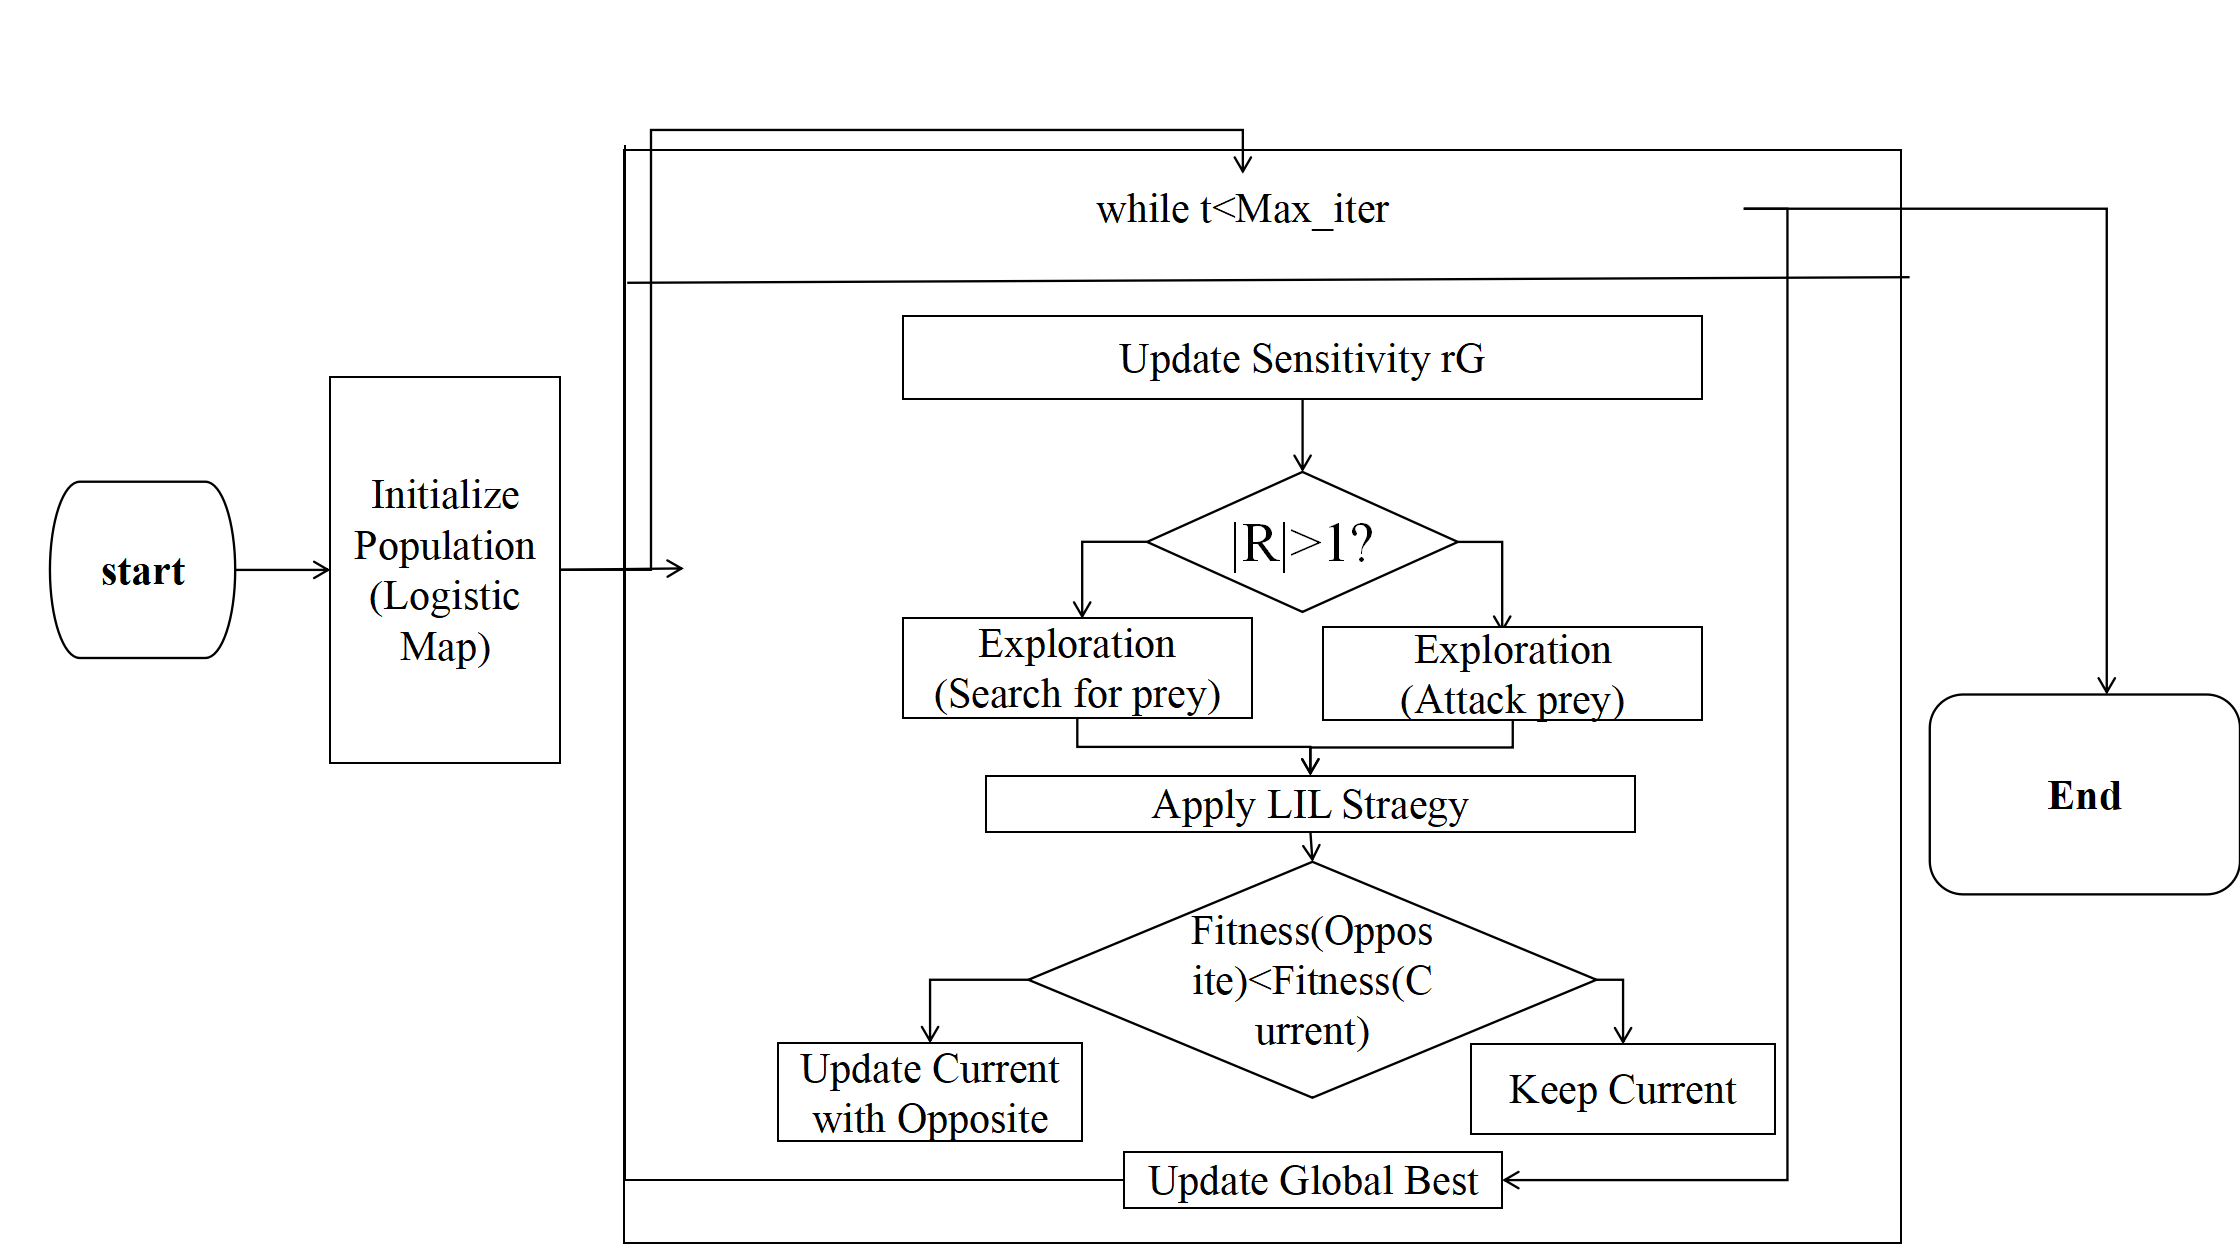
\includegraphics[width=0.9\linewidth]{optimization_flow.png}
    \caption{Flowchart of the SCSO optimization algorithm integrating the LIL strategy}
\end{figure}
The above figure provides a detailed account of the execution process of the improved SCSO algorithm after integrating the LIL strategy. The algorithm first initializes the population and then enters the main loop to simulate the sandcat's perception of the surrounding environment (carpet search) and precise attack when catching prey (local search) to update the position of the solution. The key innovation of this process lies in the introduction of a judgment branch that determines whether the current population has fallen into a local optimum (as shown in the rhombus box in the figure). Once the system detects a decrease in population diversity, it forcibly triggers the LIL strategy branch, generating an inverse solution through the lens imaging principle, thereby guiding the current population to see the global optimum solution and thus escape from the current local optimum solution. The modified path of LIL is aggregated with the regular path, and multiple population searches and optimizations are conducted until the conditions are met. The final output is the optimal VM migration scheme that meets the requirements of the lowest energy consumption and the lowest SLAV.

Although the SCSO algorithm is very good in convergence speed, when processing large-scale discrete data like cloud computing, a situation of converging too prematurely occurs\cite{aghaei2024rkan}. That is, all individuals quickly focus on a certain local optimal point. This point might have low energy consumption but a relatively high SLAV. Due to the lack of a jumping-out mechanism, the existing sand cat swarm cannot see the farther global optimal solution. regarding this situation, this research introduces the Lens Imaging Learning strategy (LIL) from optical imaging.

This strategy utilizes the reversible principle of convex lens imaging. For the current optimal solution, it produces a reverse solution\cite{bresson2024kagnns}. Mathematically, assuming this solution is $X_{best}$, then LIL calculates an $X_{nobest}$ reverse solution without exceeding the current input sequence. This reverse solution is exactly opposite to the optimal solution within the entire solution range. The deep significance of this lies in that, if the current search falls into a local optimal solution, then the opposite area might contain a better solution. LIL uses this method to force the algorithm to look at this reverse solution, thereby allowing the population to jump out of the current local optimal solution and look for the global optimal solution in the blind zone\cite{noorizadegan2025practitioner}. If the reverse solution is better than the current solution, the algorithm will choose the reverse solution, thereby realizing the escape from the local optimal solution. This mechanism expands the search surface of the population for the input sequence, thereby guaranteeing the algorithm's ability to find the global optimum. The relevant expression and relevant diagram are as follows:\begin{equation}
    X_{nobest} = \frac{lb + ub}{2} + \frac{lb + ub}{2k} - \frac{X_{best}}{k},
    \label{eq:lil_opposition}
\end{equation}where $lb$ and $ub$ represent the lower and upper bounds of the search space respectively, used to determine the geometric center of the search region, $X_{best}$ denotes the position of the current global optimal solution, and $k$ is a scaling factor controlling the perturbation step size, the formula, by combining the search space center information and subtracting the weighted influence of the current optimal solution, compels the individual to move away from the current optimal region, thereby enhancing the algorithm's global exploration capability.

\begin{figure}[!t] 
    \centering
    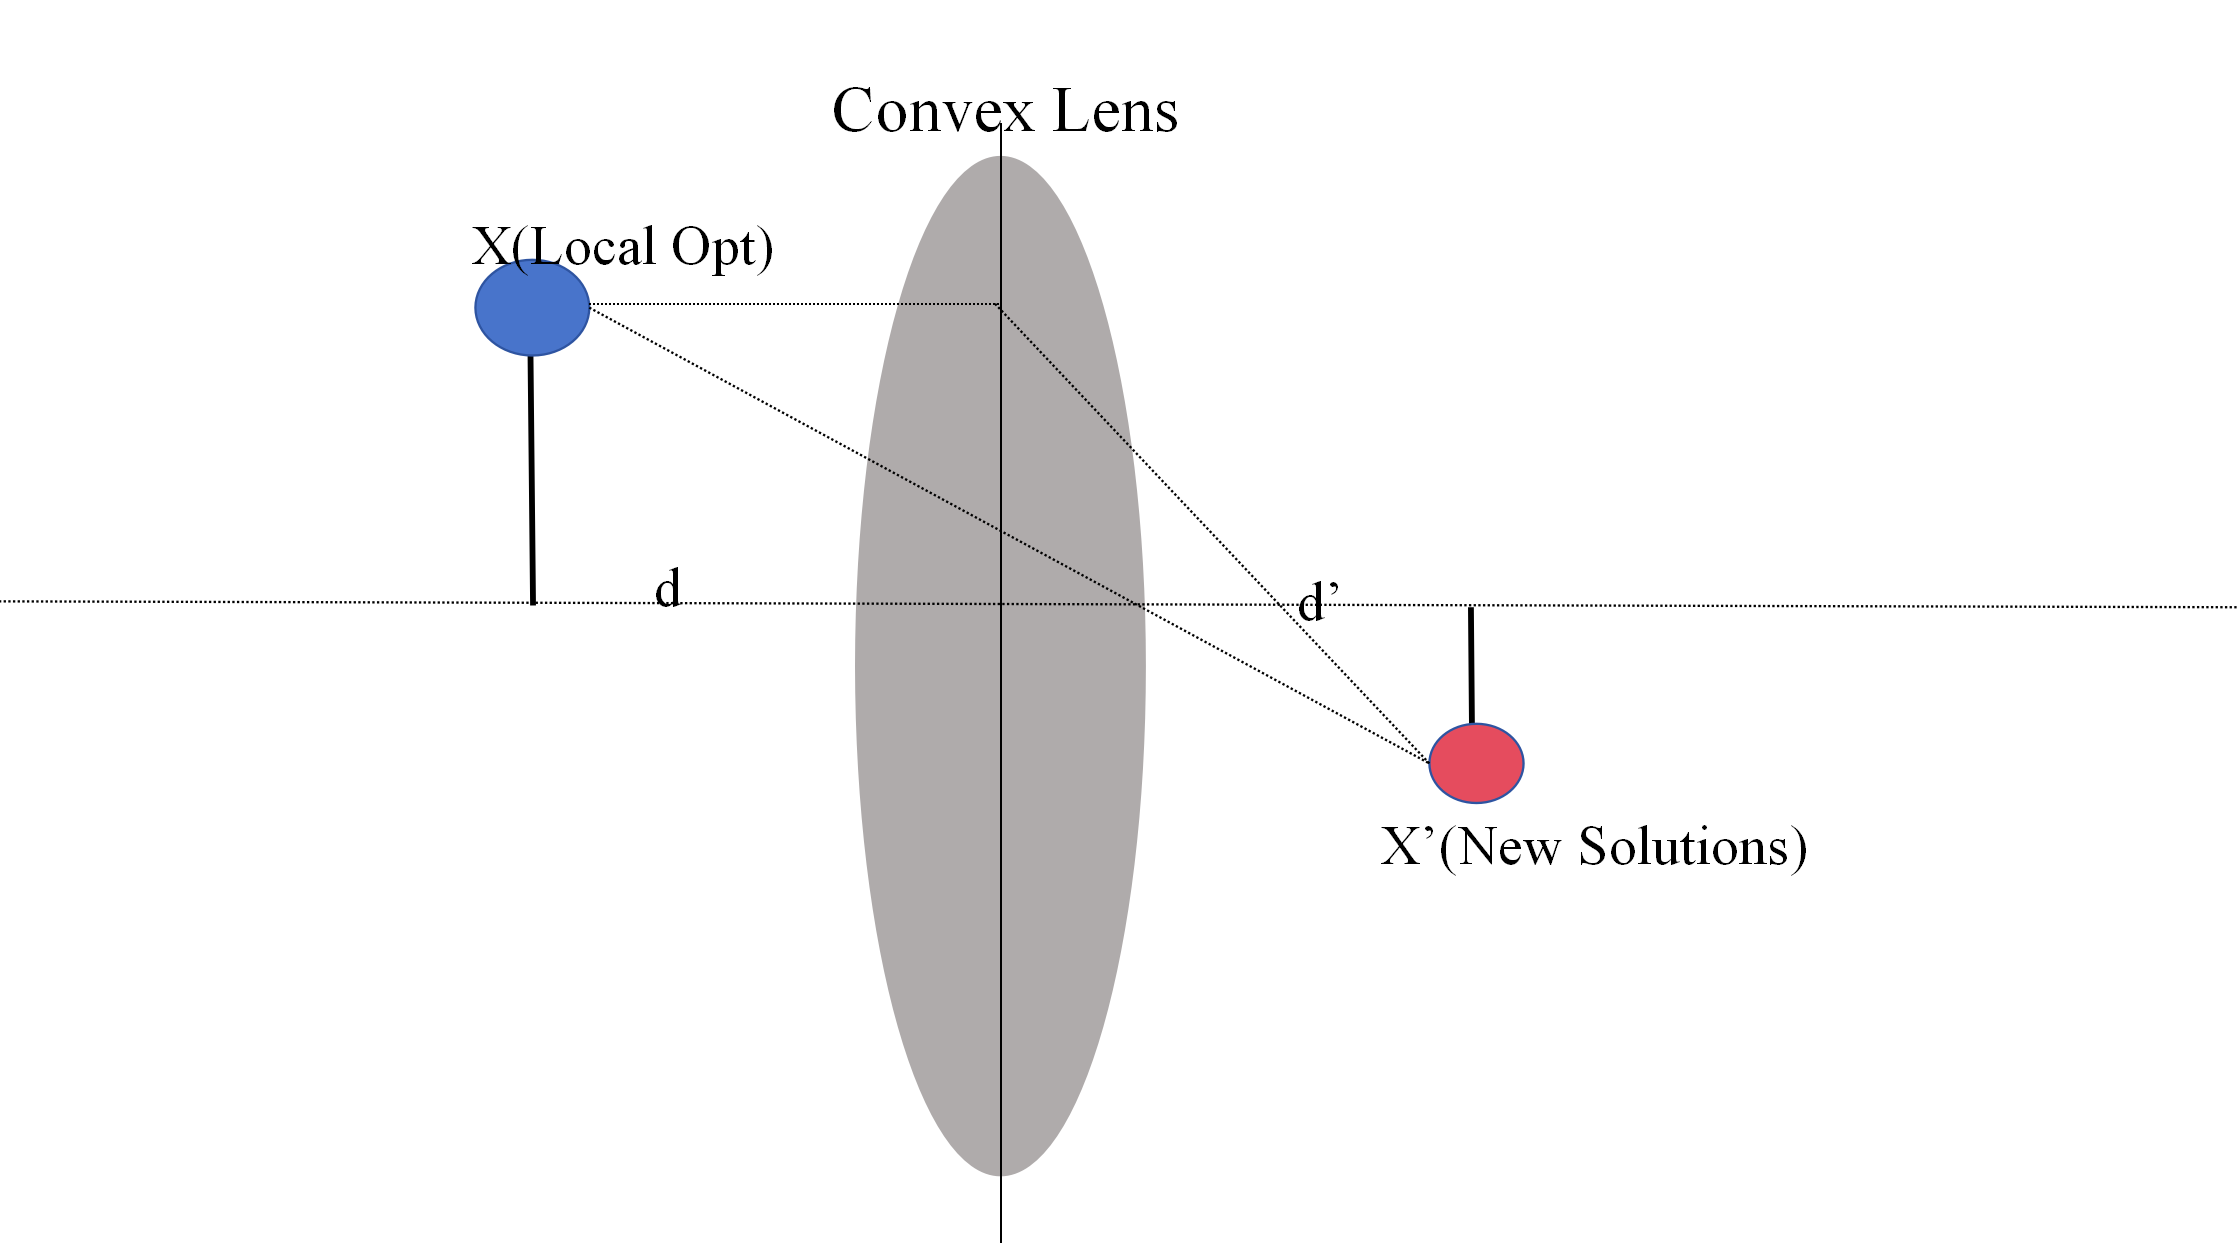
\includegraphics[width=0.9\linewidth]{fig_lil_principle.png}
    \caption{LIL Imaging Principle}
\end{figure}
The  Fig.4 intuitively analyzes the mathematical principle of the Lens Imaging Learning (LIL) strategy. During the optimization process, if the current population is already lost in the local optimal solution $X$ (the blue dot in the figure), then at this time, even producing small perturbations near $X$  does not have much effect. However, the LIL strategy is based on physical optical imaging principles. It treats $X$ as a light source, then conducts relevant refraction through the convex lens at the origin, and then produces an inverted real image $X^*$ (the small red dot in the figure) on the other side of the mirror. By changing the size of the scaling factor $k$, the algorithm can directly calculate the reverse solution that is completely opposite to the current solution. This method is actually a geometric transformation, which can help the current population take a super large-span leap when trapped in a local optimal solution, thereby being able to break free from the local optimal solution very well, and strictly increasing the probability of finding the global optimal solution to a large extent.

\begin{algorithm}[!t] 
\caption{Improved SCSO Algorithm with Lens Imaging Learning (LIL)}
\label{alg:scso_lil}
\begin{algorithmic}[1]
% --- 输入输出 ---
\State \textbf{Input:} Population size $N$, Max iterations $T_{max}$, Search boundaries $[LB, UB]$.
\State \textbf{Output:} The global best solution $X_{best}$ (Optimal VM Migration Strategy).

% --- 步骤 1: 初始化 ---
\State \textbf{Step 1: Initialization}
\State Initialize population $X_i (i=1...N)$ randomly within $[LB, UB]$;
\State Calculate fitness for all agents using Eq. (11) (Energy \& SLA);
\State Identify the current best solution $X_{best}$;

% --- 步骤 2: 主循环 ---
\State \textbf{Step 2: Main Optimization Loop}
\While{$t < T_{max}$}
    \State Update sensitivity range $r_G$ linearly from 2 to 0;
    \For{each search agent $X_i$ in population}
        \State Calculate Energy parameter $E$; \Comment{Controls search behavior}
        
        % 探索与开发
        \If{$|E| \ge 1$} 
            \State \textbf{Exploration Phase:} Update position randomly (Search for prey);
        \Else
            \State \textbf{Exploitation Phase:} Update position towards $X_{best}$ (Attack prey);
        \EndIf
        
        % --- LIL 策略 (核心改进) ---
        \State \textbf{Step 3: Lens Imaging Learning Strategy}
        \State Generate opposition solution $X'_{i}$ using LIL principle;
        \State Calculate fitness of $X'_{i}$;
        \If{$Fitness(X'_{i}) < Fitness(X_{i})$}
            \State Update $X_{i} \leftarrow X'_{i}$; \Comment{Accept better opposition solution}
        \EndIf
        
        \State Boundary check for $X_i$ to ensure validity;
    \EndFor
    
    \State Update global best $X_{best}$ if a better solution is found;
    \State $t \leftarrow t + 1$;
\EndWhile

\State \textbf{Return} $X_{best}$.
\end{algorithmic}
\end{algorithm}

In order to achieve a balance between SLA and energy consumption, SCSO-LIL does not solely pursue the minimum energy consumption, but chooses to use a weighted multi-objective fitness function. This function adds the predicted energy consumption $E_{pred}$ and the predicted default rate $SLAV_{pred}$ output by the BiTCN-Attention-KAN model in a weighted manner\cite{xu2024kolmogorov}. Setting weights can reflect the system's preference for different objectives. When the current overall load is relatively low, the energy consumption weight can be appropriately increased to pursue extreme energy saving, while during peak periods, SLA is given a higher weight to ensure stability.

More importantly, since what is input is the predicted value rather than the current value, this function guides the algorithm to look for a situation where future overall resources are better\cite{hidayat2024machine}. This represents that the algorithm favors those safe solutions (insurance solutions) that have low energy consumption and are not so prone to overload in the future, thereby avoiding repeated migration caused by only seeing the current optimum.
\begin{equation}
    \text{Minimize } F = \alpha \cdot E_{total}^{pred} + \beta \cdot SLAV^{pred},
    \label{eq:fitness_function}
\end{equation}
where $E^{pred}_{total}$ and $SLAV^{pred}$ represent the predicted total energy consumption of the data center and the Service Level Agreement violation rate respectively, serving as the two core metrics for evaluating the quality of scheduling schemes, while $\alpha$ and $\beta$ are weighting coefficients used to regulate the relative importance of these two aspects during the optimization process, thereby guiding the algorithm to minimize negative impacts on service quality while reducing energy consumption.

\subsection{Algorithm Implementation Steps}

Due to the change of time, the initial VMM scheme with the fluctuation of workload causes part of the physical machine overload problem, which can lead to SLA violations, further contributing to the rise of overall energy consumption of data centers and QoS degradation. For this reason, we make use of dynamic migration algorithm to transfer the VMs of the overloaded physical machine to the physical machine with currently lower energy consumption, so as to achieve the reduction of overall energy consumption. The BiTCN-Attention-KAN model checks the status of all physical machines in the data center against a set maximum energy consumption threshold $EC\_{max}$ to periodically and dynamically migrate VMs to target physical machines.

In order to determine the physical machine energy consumption threshold, we leveraged the methodology of related research, i.e., we take the top 90\% of the physical machines with the highest energy consumption as the servers that require moving out of the VMs, which of them is selected the lowest value of the energy consumption as the current maximum physical machine energy consumption threshold. This migration method effectively obtains the physical machines with the lowest energy consumption to house the VMs. Those VMs with the lowest CPU usage among physical machines that exceed the maximum energy consumption threshold can be determined to be migrated. We take advantage of the SCSO-LIL algorithm to move out to the target physical machine, which is less than the maximum energy consumption threshold. In other words, multiple VMs are migrated to the physical machines with the lowest energy consumption.


\section{experiment and result analysis}

\begin{table}[t!]
\centering
\caption{Simulation Parameters and Algorithm Settings}
\label{tab:experiment_parameters}
% --- 核心修改：用 resizebox 包裹整个 tabular ---
% \linewidth 表示缩放到当前栏宽，! 表示高度自动保持比例
\resizebox{\linewidth}{!}{ 
    \setlength{\tabcolsep}{2mm} % 稍微减小间距
    \renewcommand{\arraystretch}{1.2}
    \begin{tabular}{ll}
    \toprule
    \textbf{Parameter} & \textbf{Value / Specification} \\
    \midrule
    \multicolumn{2}{l}{\textbf{\textit{1. Cloud Data Center Settings}}} \\
    Simulation Platform & Cloudsim 3.0.3 \\
    PM Number & 800 (Heterogeneous) \\
    PM Types & HP ProLiant G4, G5 \\ % 稍微缩短文字
    VM Number & 1052 \\
    VM MIPS & 500, 1000, 1500, 2000, 2500 \\
    RAM Capacity & 4 GB (PMs), 512MB-2.5GB \\ % 稍微缩写
    Bandwidth & 1 Gbit/s \\
    Energy Consumption Trace & PlanetLab (20110303) \\
    Scheduling Interval & 300 s \\
    Power Model & SpecPower Benchmark \\
    \midrule
    \multicolumn{2}{l}{\textbf{\textit{2. BiTCN-Attention-KAN Model}}} \\
    Input Sliding Window & 12 (History steps) \\
    Prediction Horizon & 1 (Next step) \\
    Convolutional Kernels & 64 \\
    Dilation Factors & [1, 2, 4, 8] \\
    KAN Grid Size & 5 \\
    KAN Spline Order & 3 \\
    Batch Size & 64 \\
    Learning Rate & 0.001 (Adam) \\
    Training Epochs & 100 \\
    \midrule
    \multicolumn{2}{l}{\textbf{\textit{3. SCSO-LIL Algorithm}}} \\
    Population Size ($N$) & 30 \\
    Max Iterations & 1000 \\
    Sensitivity ($r_G$) & Linear: 2 to 0 \\ % 缩写
    Lens Scaling ($k$) & 100 \\
    Energy Weight ($\alpha$) & 0.6 \\
    SLA Weight ($\beta$) & 0.4 \\
    Independent Runs & 30 \\
    \bottomrule
    \end{tabular}
} % resizebox 结束的大括号
\end{table}

\subsection{Experimental setup}

Cloudsim 3.0.3 is chosen as the simulation platform for the experiment, mainly because this platform has its own architecture for discrete case simulation. This architecture accurately obtains the subtle changes of VMs during migration. Moreover, this platform also supports interfaces that are customized to adjust energy consumption, which is very important for verifying energy consumption optimization in various situations. In reality, cloud loads generally have unpredictable traffic compared to artificially synthesized data. The data contains fluctuating data with periodic changes and randomly occurring energy consumption values that are difficult to predict. This complex situation can test the model's predictive ability in various circumstances. Moreover, before the data is input into the model, it is uniformly processed to reduce the impact of numerical differences caused by different PMs.

Two publicly published real datasets were used to evaluate the effectiveness of the BAK-SCSO-VMM algorithm. They are described below:

\begin{itemize}
\item\textbf{PlanetLab Data:}: This workload trace is provided as part of the CoMon project, a monitoring infrastructure for PlanetLab. In this project, the CPU utilization data of more than a thousand VMs from servers located at more than 500 places around the world are recorded every 5 minutes for 24 hours. During the experiment, we randomly chose the workload trace of 10 days in March and April 2011.

\item \textbf{Google Cluster Data (GCD):} This workload trace was released by Google in May 2011. It contains the usage information of machines in a Google cluster for 29 days. We extracted the task usage table, which contains the resource usage of tasks (e.g., CPU rate, memory usage, etc.) over time. In our experiments, we use the CPU usage data of 1,000 tasks over a 24-hour period.  

\end{itemize}

\subsection{Comparison algorithm}

We intended to compare BAK-SCSO-VMM with the following six compared models and algorithms to verify the superiority of the BAK-SCSO-VMM approach in optimizing data center energy consumption and SLA guarantees.

\begin{itemize}

\item \textbf{First Fit(FF):} The default scheduling policy of the Cloudsim platform, which represents a passive response mode without any predictive situations. The performance data of this are used as the baseline model of this experiment to evaluate the effect brought about by the introduction of the prediction model.

\item \textbf{EIM:} EIM is an algorithm based on a single-hidden layer feedforward neural network. It randomly initializes input layer weights and only analytically solves for the output layer weights, thus possessing extremely fast training speed. However, due to the randomness of its parameter initialization, the model often lacks generalization ability and prediction stability when facing cloud data center workloads with high nonlinearity and volatility.

\textbf{Vanilla-RNN:} Vanilla-RNN is a recurrent neural network for processing sequential data, which passes the hidden state of the previous time step to the current time step through recurrent units, thereby capturing temporal dependencies. However, due to its relatively simple network structure, it is prone to encountering vanishing gradient or exploding gradient problems during the training process, leading to difficulties in effectively capturing long-term dependencies in long sequence workloads and limiting prediction accuracy.

\item \textbf{LSTM:} LSTM is a variant designed to solve the RNN vanishing gradient problem. It introduces a gating mechanism (input gate, forget gate, and output gate) to regulate the information flow, thereby enabling it to effectively maintain and forget information in long sequences. Although LSTM performs excellently in capturing long-term dependencies, its complex internal structure leads to high computational overhead, and its serial processing manner limits parallel computing capability and training efficiency.

\item \textbf{TCN:} TCN is an architecture based on causal dilated convolution, combining the parallel computing advantages of convolutional neural networks with sequence modeling capabilities. By stacking dilated convolution layers and residual connections, TCN is able to obtain an extremely large receptive field with fewer parameters, thereby effectively capturing local sudden changes and global trends of workload data, and avoiding the vanishing gradient problem of RNN.

\item \textbf{BiTCN:} BiTCN introduces a bi-directional structure on the basis of TCN, extracting temporal features from both forward and backward dimensions simultaneously. This mechanism allows the model not only to utilize past historical workload information but also to combine the overall contextual background of the sequence. Compared with unidirectional models, BiTCN can more comprehensively extract deep features under complex workload patterns, thereby further improving the prediction robustness of the model for high loads and burst traffic.
\end{itemize}

The evaluation indicators selected are some major issues that the data center pays attention to during operation: energy consumption, SLAV and the number of migrations. Energy consumption is directly related to the cost during operation, while the number of migrations represents the accuracy of the prediction results, and SLAV is an indicator that can directly reflect the user experience. The ability to maintain a low SLAV while reducing energy consumption is a key criterion for evaluating whether an algorithm is good or not.
\begin{figure}[htbp]
    \centering
    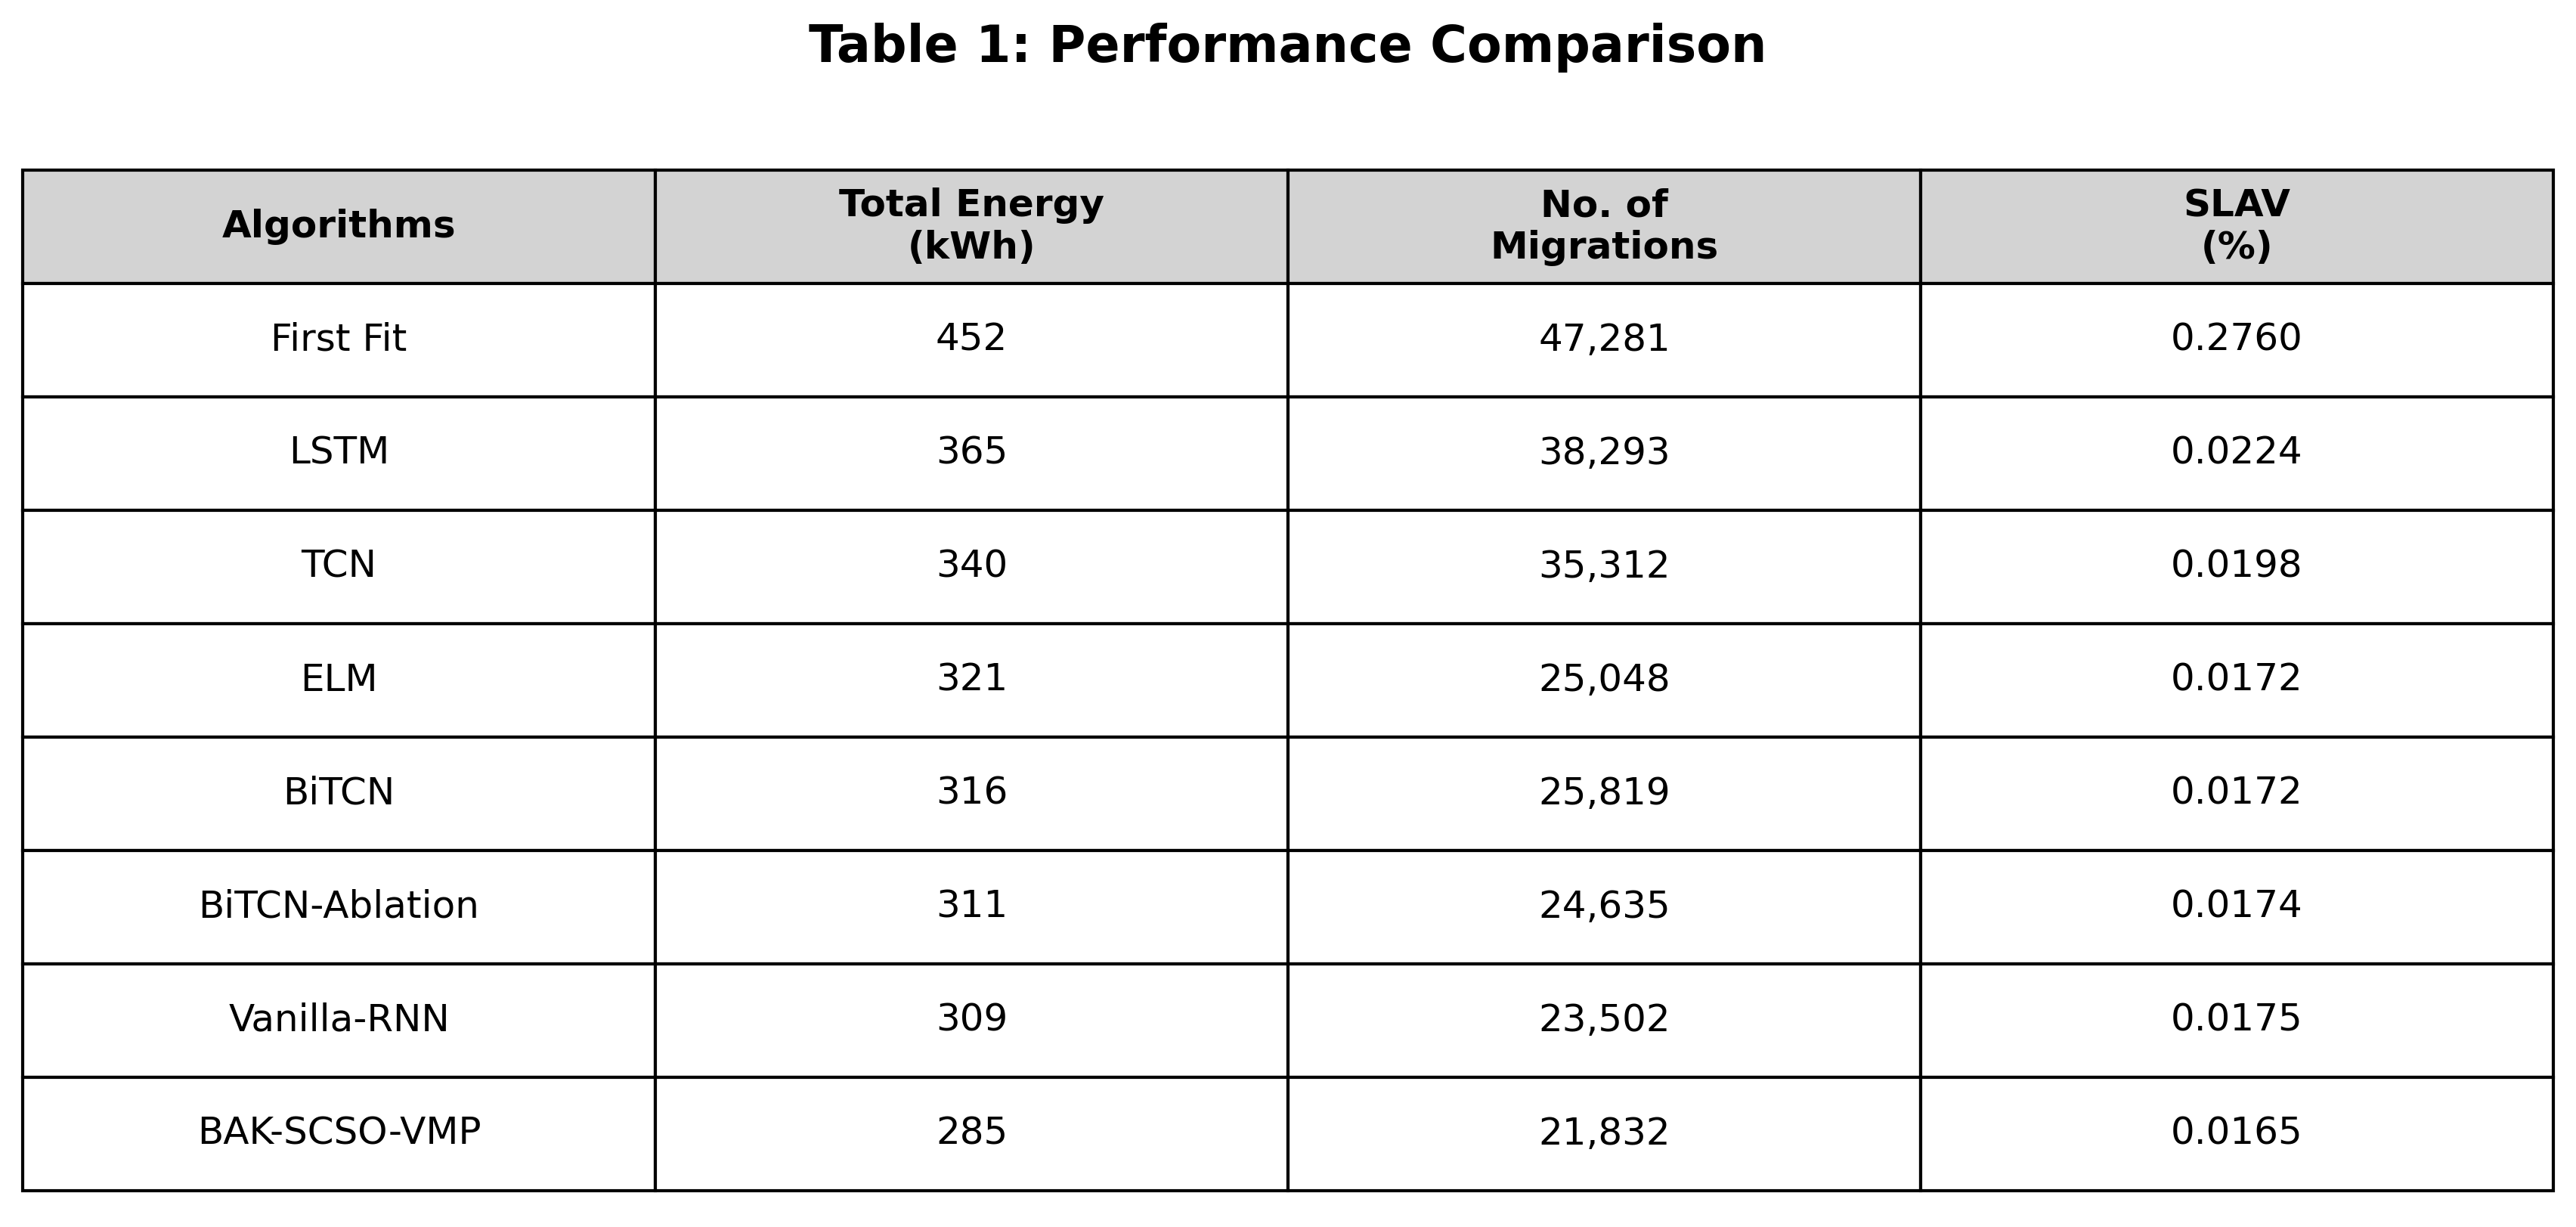
\includegraphics[width=0.95\linewidth]{tab_performance.png}
    \caption{A performance comparison data table of each algorithm in terms of energy consumption, migration times and SLA default rate}
\end{figure}
\subsection{Energy consumption analysis}
\begin{figure}[H]   % <--- 改成 [H]
    \centering
    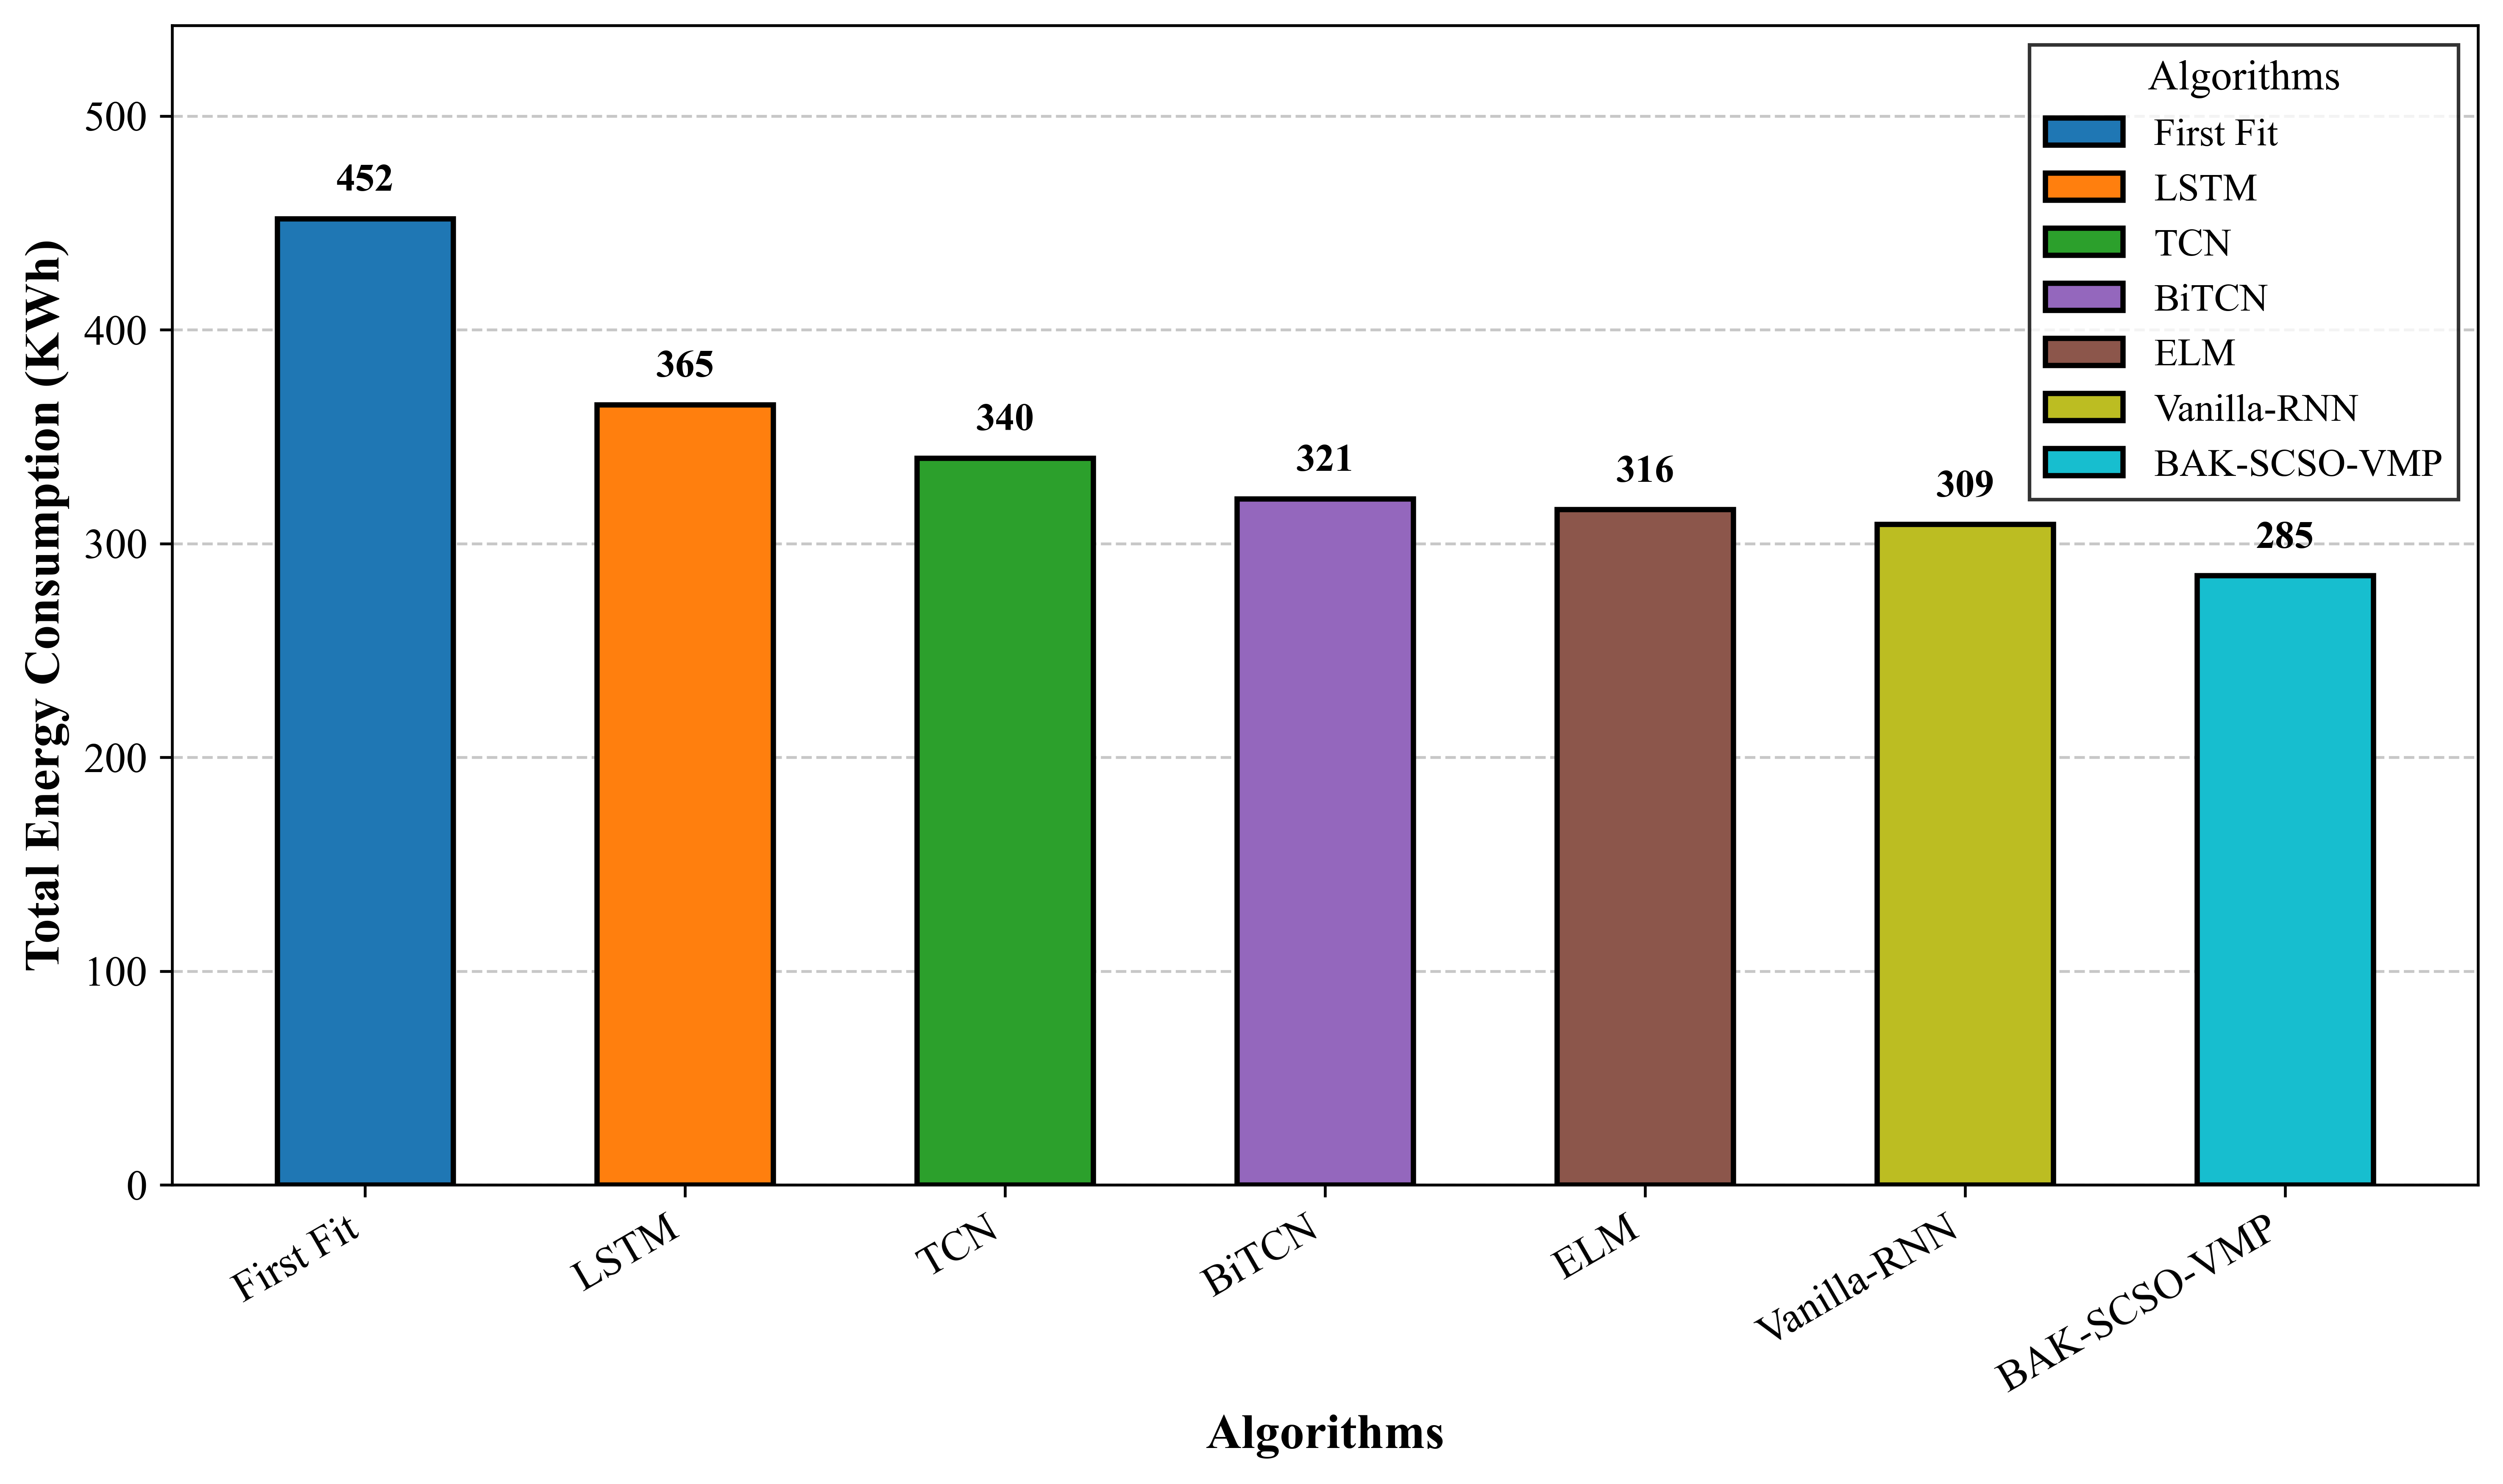
\includegraphics[width=0.65\linewidth]{fig_energy.png}
    \caption{Comparison of total energy consumption under different algorithms}
    \label{fig:energy}
\end{figure}It can be seen from the figure that the reason for the high energy consumption of 452KWh of FirstFit lies in the excessive integration strategy. Due to the lack of prediction for future loads, the FirstFit algorithm tends to keep many PMs in standby mode to ensure timely response when requests arrive. According to the energy consumption model, even if the PM is in an idle state, the power consumption still reaches about 70\% of the maximum value. This ineffective large number of hole piles is the key reason why the energy consumption remains at a high level and cannot be reduced.
Relatively speaking, the method of this study can reduce energy consumption to 285KWh. The key to this lies in the early perception of the drawbacks caused by the overly integrated strategy. Thanks to the accurate prediction of the BiTCN-Attention-KAN model, the system is able to promptly identify the PMs that may be under low load for a long time in the future. The SCSO-LIL scheduling strategy performs scheduling operations based on this prediction, resolutely migrating VMs from the PM, thereby enabling more physical machines (PMs) to enter sleep mode in a timely manner.

Even the BiTCN model (316KWh), which also has predictive capabilities, still consumes about 10\% more energy than the method in this study. This also reflects from the side the difference in the ability to predict data accuracy. When the BiTCN model is confronted with nonlinear load energy consumption curves, the prediction results usually tend to adopt very conservative strategies, which leads the scheduling algorithm to be reluctant to reduce resources to the extreme. After integrating Attention-KAN, the model has a stronger ability to approximate some more complex curves, and can more accurately improve the smoothness of the curves, thereby giving the scheduling algorithm confidence to further migrate VMs when dealing with fluctuating curves to reduce energy consumption.

\subsection{Analysis of Migration Frequency}
\begin{figure}[H]   % <--- 改成 [H]
    \centering
    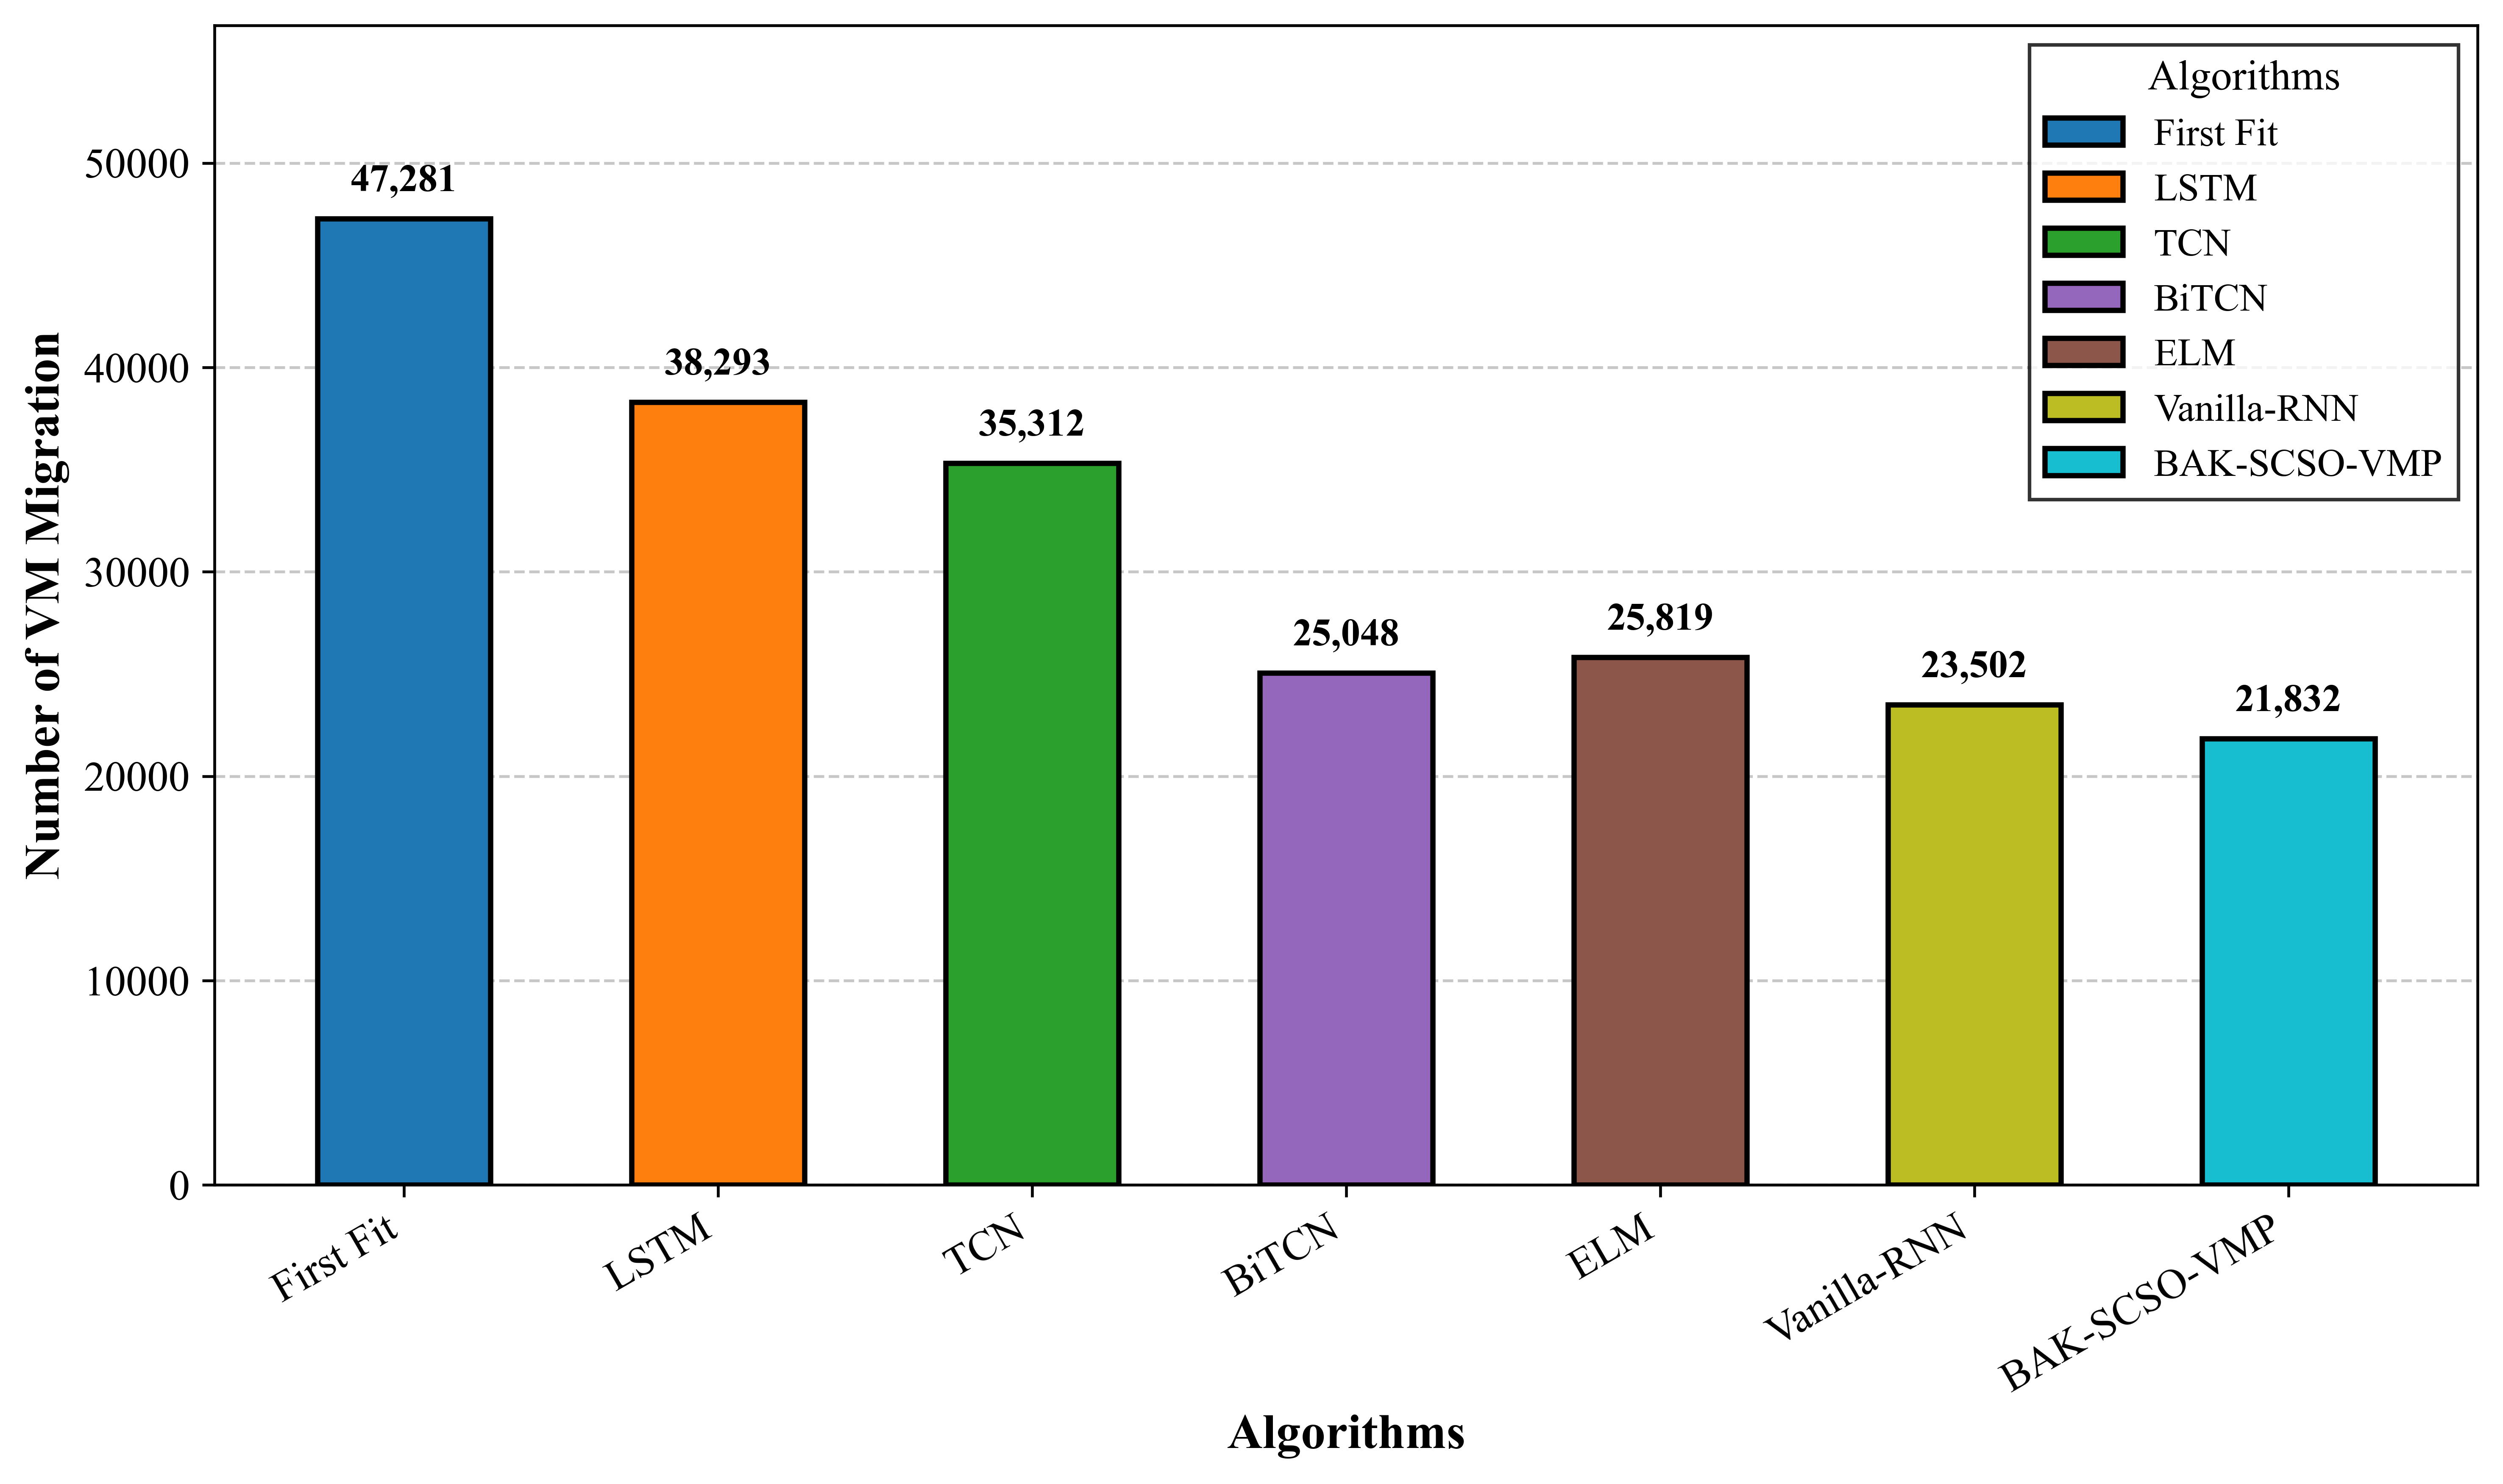
\includegraphics[width=0.85\linewidth]{fig_migration.png}
    \caption{Comparison of cumulative VM migrations for each algorithm}
    \label{fig:migration}
\end{figure}
As can be seen from the figure, the First Fit algorithm migrates VMs up to 47,281 times, and the number of migrations is related to the stability of the system when facing dynamic loads. The fewer migrations there are, the stronger the stability of the system is. However, the number of migrations of First Fit is too high, reflecting a constantly swinging situation when there is no predictive model. Due to the lack of a predictive model to assist, the algorithm is affected by sudden load fluctuations. For instance, if the energy consumption is high at one moment, the VM is migrated out, and if the energy consumption is low at the next moment, the VM is migrated back. Such frequent scheduling operations lead to a further increase in the energy consumption of the PM.

The method of this study reduced the number of migrations to 21,832, mainly thanks to optimizations in two aspects. First, the prediction results of the BiTCN-Attention-KAN model filter out some results. For instance, when the load fluctuates for a very short period of time, the model determine whether this is a continuous upward or downward change by combining previous data. If it is judged not to be so, it is ignored. This reduces the excessive migration of the scheduling algorithm, thereby avoiding unnecessary migrations. Secondly, the SCSO-LIL optimization algorithm adopts a global aspect search strategy. Unlike the common greedy strategy, SCSO-LIL considers the algorithm from multiple perspectives, thereby seeking a migration strategy that can remain stable for a long time in the future. This one-step VM migration method directly avoids the situation where a secondary migration is required due to resource competition later on. This reflects the key idea of this study, which is to reduce the frequency of operations by upgrading the quality of decisions.
\subsection{SLAV Analysis}
\begin{figure}[H] 
    \centering
    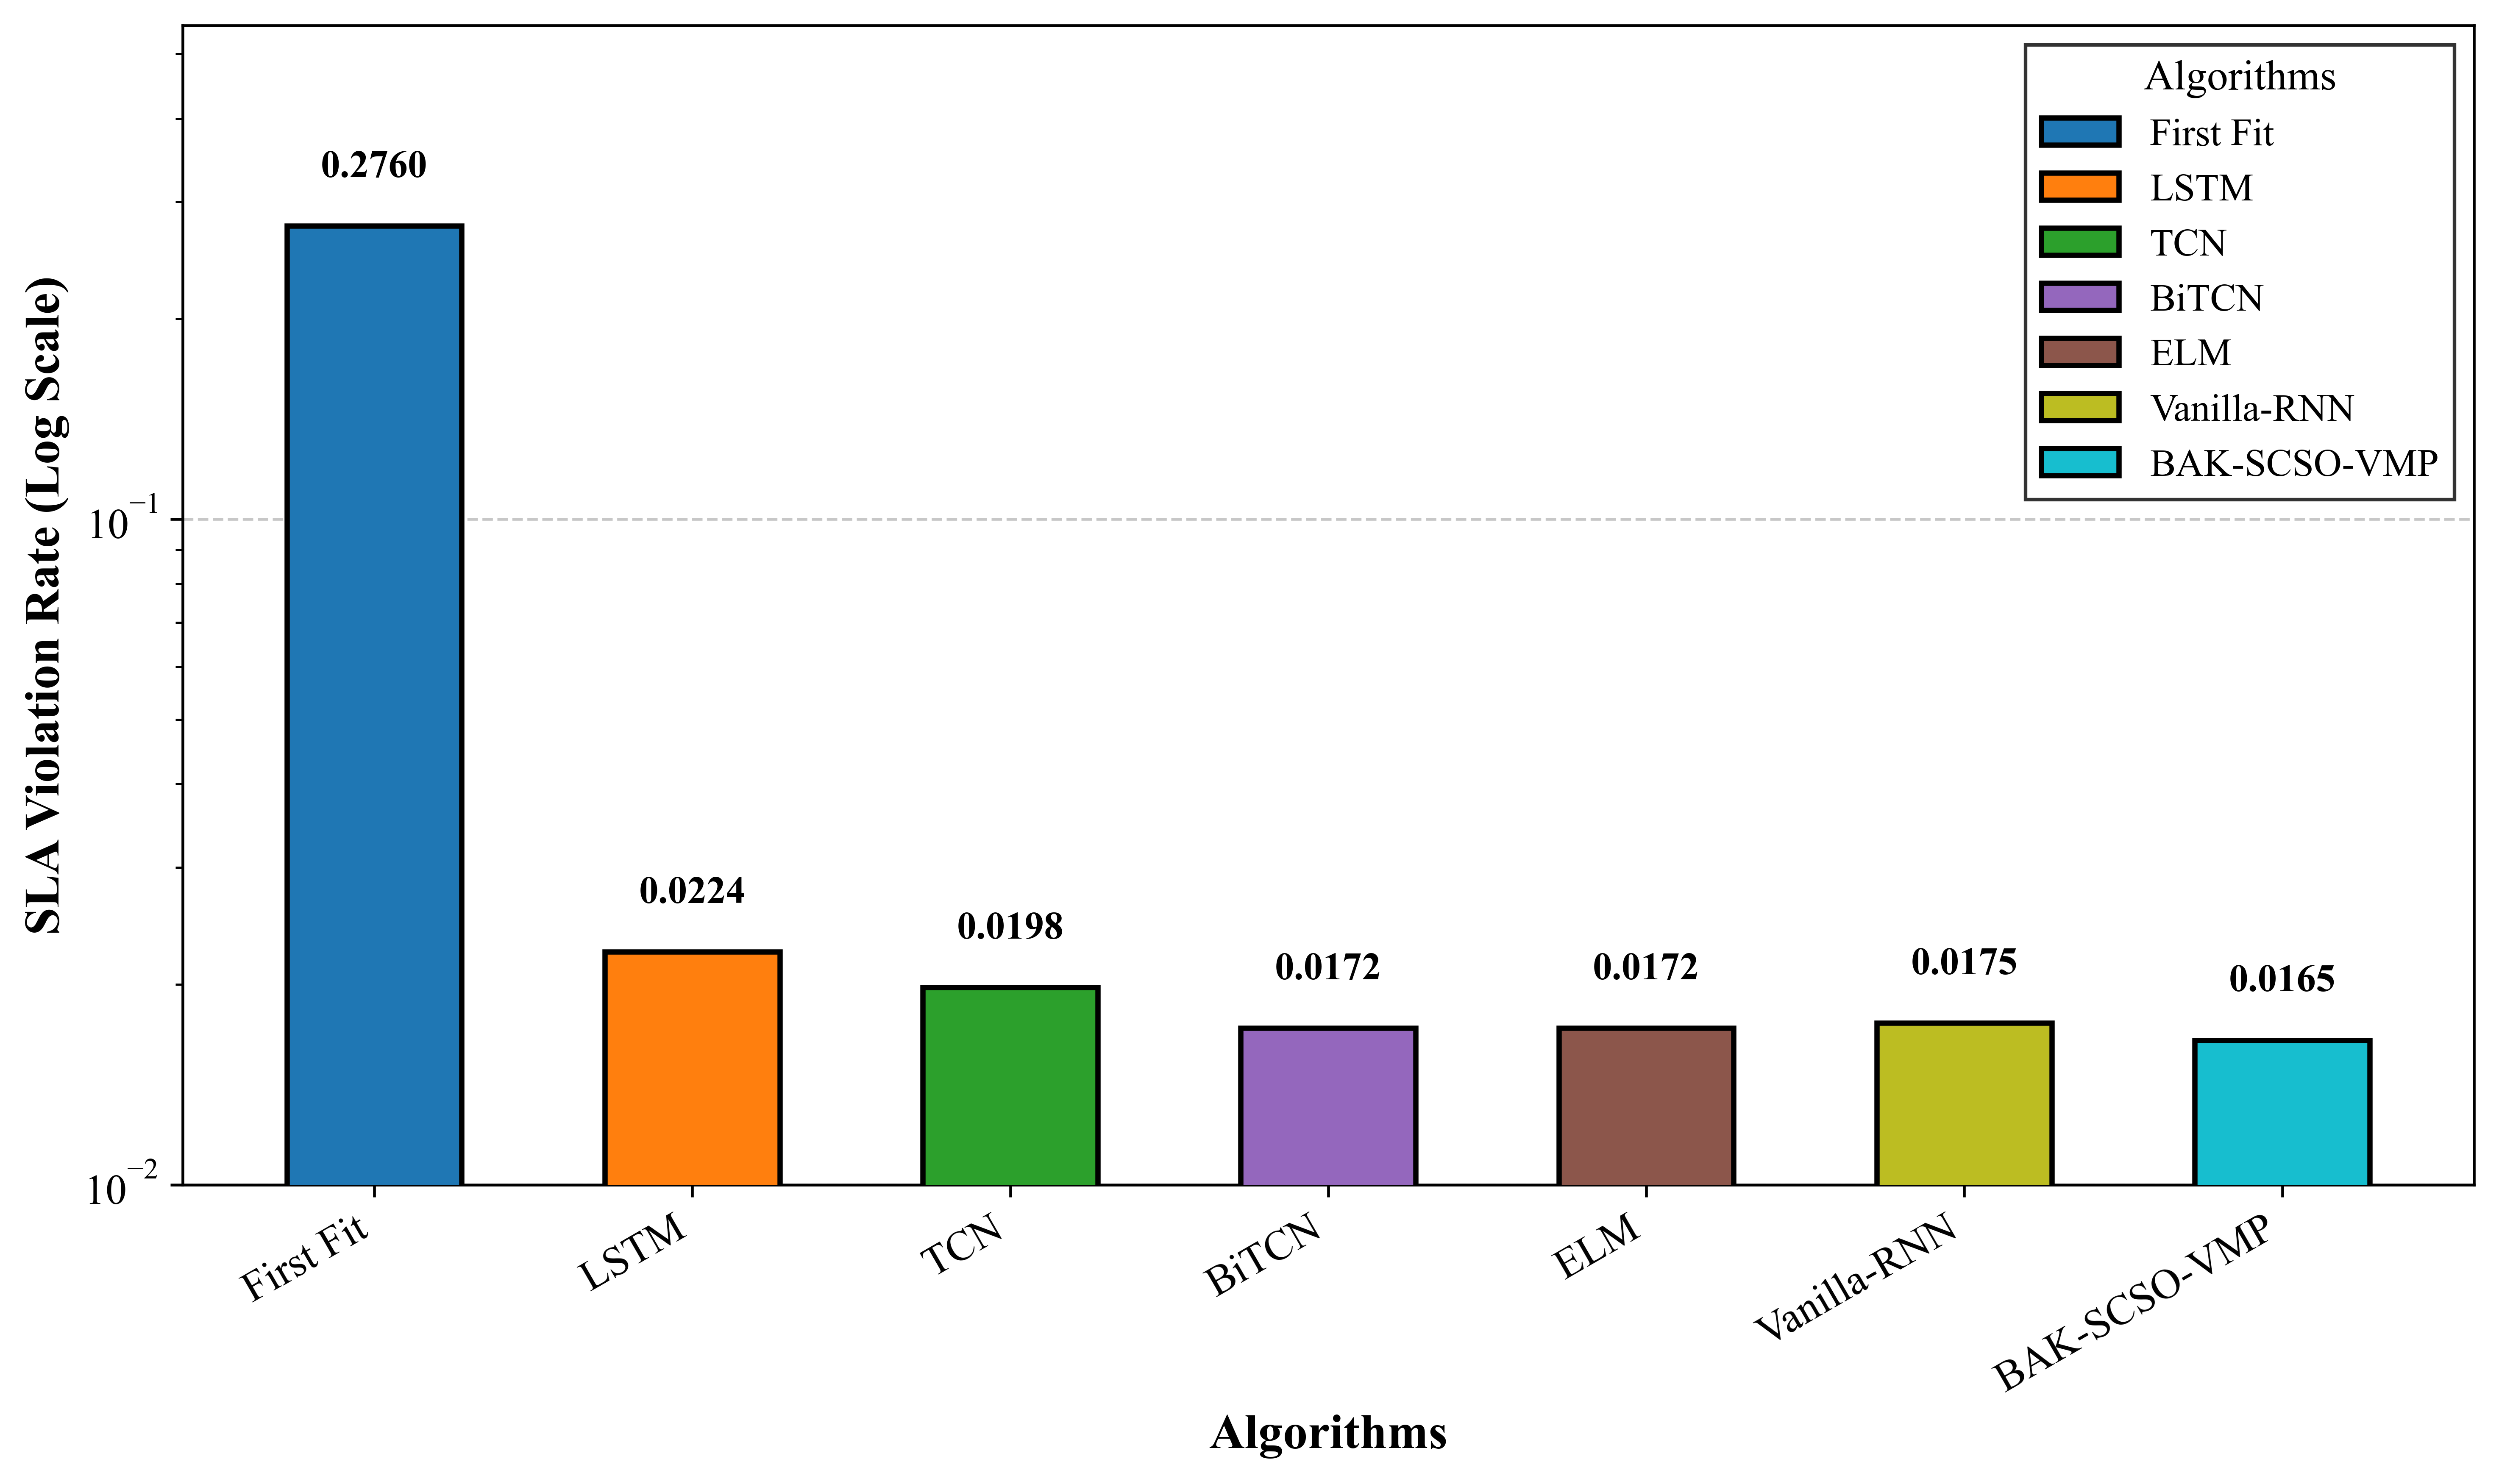
\includegraphics[width=0.85\linewidth]{fig_sla.png}
    \caption{SLA Violation Rate Comparison}
    \label{fig:SLA}
\end{figure}
As can be seen from the figure, the SLAV has decreased from 0.0276 \% to 0.0165 \%. This improvement reflects the reliability of the system under extreme conditions. The high default rate of First Fit is caused by the random allocation of resources. If the FirstFit algorithm blindly pursues high integration, it strives to fill up the PM. However, if multiple VMs simultaneously request resources at the same time, it causes the PM resources to be consumed all at once, resulting in multiple requests having to be queued, which in turn leads to a breach of SLA.

This method ensures the lowest energy consumption while also guaranteeing the lowest default rate. This may seem contradictory, but in fact, it is all thanks to the strategy of early migration. Attention-KAN plays an important role in it. It can accurately identify the key time series where the load changes suddenly. Before the actual load peak arrives, the system has already completed the policy provision in advance. According to this strategy, the SCSO-LIL scheduling algorithm migrates some critical tasks in advance from some PMs with high load risks to some nodes with low energy consumption. This preventive strategy in advance can effectively avoid the occurrence of resource congestion.

In addition, the low default rate of 0.0165 \% also simultaneously demonstrates the advantages of this algorithm. Even in the face of a simulated real environment like PlanetLab, which contains a lot of uncertain and unpredictable data, this method can accurately find the optimal balance point between low energy consumption and low default rate. Experimental data show that the  model successfully solves the problem of being unable to take into account both energy consumption and SLA simultaneously by combining the Attention-KAN and SCSO-LIL algorithms, which have a higher approximation ability for nonlinear curves.
% An example of a floating figure using the graphicx package.
% Note that \label must occur AFTER (or within) \caption.
% For figures, \caption should occur after the \includegraphics.
% Note that IEEEtran v1.7 and later has special internal code that
% is designed to preserve the operation of \label within \caption
% even when the captionsoff option is in effect. However, because
% of issues like this, it may be the safest practice to put all your
% \label just after \caption rather than within \caption{}.
%
% Reminder: the "draftcls" or "draftclsnofoot", not "draft", class
% option should be used if it is desired that the figures are to be
% displayed while in draft mode.
%
%\begin{figure}[!t]
%\centering
%\includegraphics[width=2.5in]{myfigure}
% where an .eps filename suffix will be assumed under latex, 
% and a .pdf suffix will be assumed for pdflatex; or what has been declared
% via \DeclareGraphicsExtensions.
%\caption{Simulation results for the network.}
%\label{fig_sim}
%\end{figure}

% Note that the IEEE typically puts floats only at the top, even when this
% results in a large percentage of a column being occupied by floats.


% An example of a double column floating figure using two subfigures.
% (The subfig.sty package must be loaded for this to work.)
% The subfigure \label commands are set within each subfloat command,
% and the \label for the overall figure must come after \caption.
% \hfil is used as a separator to get equal spacing.
% Watch out that the combined width of all the subfigures on a 
% line do not exceed the text width or a line break will occur.
%
%\begin{figure*}[!t]
%\centering
%\subfloat[Case I]{\includegraphics[width=2.5in]{box}%
%\label{fig_first_case}}
%\hfil
%\subfloat[Case II]{\includegraphics[width=2.5in]{box}%
%\label{fig_second_case}}
%\caption{Simulation results for the network.}
%\label{fig_sim}
%\end{figure*}
%
% Note that often IEEE papers with subfigures do not employ subfigure
% captions (using the optional argument to \subfloat[]), but instead will
% reference/describe all of them (a), (b), etc., within the main caption.
% Be aware that for subfig.sty to generate the (a), (b), etc., subfigure
% labels, the optional argument to \subfloat must be present. If a
% subcaption is not desired, just leave its contents blank,
% e.g., \subfloat[].


% An example of a floating table. Note that, for IEEE style tables, the
% \caption command should come BEFORE the table and, given that table
% captions serve much like titles, are usually capitalized except for words
% such as a, an, and, as, at, but, by, for, in, nor, of, on, or, the, to
% and up, which are usually not capitalized unless they are the first or
% last word of the caption. Table text will default to \footnotesize as
% the IEEE normally uses this smaller font for tables.
% The \label must come after \caption as always.
%
%\begin{table}[!t]
%% increase table row spacing, adjust to taste
%\renewcommand{\arraystretch}{1.3}
% if using array.sty, it might be a good idea to tweak the value of
% \extrarowheight as needed to properly center the text within the cells
%\caption{An Example of a Table}
%\label{table_example}
%\centering
%% Some packages, such as MDW tools, offer better commands for making tables
%% than the plain LaTeX2e tabular which is used here.
%\begin{tabular}{|c||c|}
%\hline
%One & Two\\
%\hline
%Three & Four\\
%\hline
%\end{tabular}
%\end{table}


% Note that the IEEE does not put floats in the very first column
% - or typically anywhere on the first page for that matter. Also,
% in-text middle ("here") positioning is typically not used, but it
% is allowed and encouraged for Computer Society conferences (but
% not Computer Society journals). Most IEEE journals/conferences use
% top floats exclusively. 
% Note that, LaTeX2e, unlike IEEE journals/conferences, places
% footnotes above bottom floats. This can be corrected via the
% \fnbelowfloat command of the stfloats package.

\section{Conclusion}

This paper proposes a  active resource management framework based on deep learning prediction and group scheduling to address the contradiction between excessive energy consumption and service level agreement (SLA) default rate that may occur in cloud data centers when dealing with dynamic loads related to cloud computing. This framework achieves high-precision prediction of complex nonlinear energy consumption through the BiTCN-Attention  model, thereby overcoming the linear output limitation of the LSTM model in the face of sudden changes in energy consumption. Moreover, it combines the lens imaging Learning (LIL) strategy to improve the Sandcat swarm optimization algorithm (SCSO). The problem of easily getting stuck in local optima when placing a large number of virtual machines has been solved.
% conference papers do not normally have an appendix


% use section* for acknowledgment
\section*{Acknowledgment}


The authors would like to thank...





% trigger a \newpage just before the given reference
% number - used to balance the columns on the last page
% adjust value as needed - may need to be readjusted if
% the document is modified later
%\IEEEtriggeratref{8}
% The "triggered" command can be changed if desired:
%\IEEEtriggercmd{\enlargethispage{-5in}}

% references section

% can use a bibliography generated by BibTeX as a .bbl file
% BibTeX documentation can be easily obtained at:
% http://mirror.ctan.org/biblio/bibtex/contrib/doc/
% The IEEEtran BibTeX style support page is at:
% http://www.michaelshell.org/tex/ieeetran/bibtex/
%\bibliographystyle{IEEEtran}
% argument is your BibTeX string definitions and bibliography database(s)
%\bibliography{IEEEabrv,../bib/paper}
%
% <OR> manually copy in the resultant .bbl file
% set second argument of \begin to the number of references
% (used to reserve space for the reference number labels box)

\bibliographystyle{unsrt}
 \bibliography{IEEEexample}

% that's all folks
\end{document}


